\secnumbersection{VALIDACIÓN DE LA SOLUCIÓN}

Esta sección valida empíricamente DRAFTS++ mediante casos de uso que demuestran funcionalidad, robustez temporal y escalabilidad, además de evaluar estrategias de detección en alta frecuencia (86 GHz).

% La metodología de validación implementada sigue un enfoque sistemático y comparativo que garantiza la reproducibilidad de los resultados. Para cada componente, se establecieron métricas de evaluación específicas, se utilizaron datasets de referencia validados por la literatura científica, y se implementaron protocolos de verificación independientes con grupos de astrónomos colaboradores.

% Los objetivos principales de esta validación incluyen: (1) demostrar la superioridad de los pipelines desarrollados respecto a métodos existentes, (2) validar la capacidad de procesamiento de archivos de gran tamaño, (3) confirmar la precisión temporal y espacial en la detección de eventos, (4) evaluar la eficiencia computacional y escalabilidad del sistema, y (5) establecer la capacidad de descubrimiento científico mediante la detección de eventos nuevos no reportados previamente en la literatura.

\subsection{VALIDACIÓN DEL COMPONENTE 1: DRAFTS++ - Pipeline astronómico E2E, Productivo, Robusto y Eficiente}

La validación utiliza tres casos progresivos que ejercitan las siete etapas del pipeline (Figura~\ref{fig:workflow-src}) bajo complejidad creciente:

\begin{enumerate}
    \item \textbf{FAST-FREX (Radiotelescopio FAST)}: Dataset de entrenamiento del Five-hundred-meter Aperture Spherical Telescope (FAST, China) que valida flujo completo E2E con modelos CenterNet/ResNet18 integrados. Formato PSRFITS, frecuencia central $\sim$1.25 GHz.
    
    \item \textbf{Pulsar B0355+54 (Radiotelescopio FAST)}: Observación de 117s del radiotelescopio FAST conteniendo 752 pulsos teóricos del púlsar B0355+54 (periodo 0.156s) que valida streaming, continuidad temporal y trazabilidad (732/752 detectados, 97.3\%). Formato PSRFITS.
    
    \item \textbf{FRB 121102 (Radiotelescopio Effelsberg)}: 6 archivos de observación del radiotelescopio Effelsberg de 100m (Alemania) en banda L ($\sim$1.4 GHz), cada uno de $\sim$4 GB, que validan escalabilidad, gestión de memoria y descubrimiento científico (Recall 100\%, 2 nuevos bursts). Datos reportados por \cite{cruces2020frb121102}.
\end{enumerate}

El éxito en los tres casos demuestra que todas las etapas del pipeline operan coordinadamente. Cualquier falla en etapas principales o módulos de soporte causaría fallos completos del sistema.

\begin{table}[H]
\centering
\caption{Mapeo entre etapas del pipeline DRAFTS++ y casos de validación implementados. Cada caso ejercita múltiples etapas de manera integrada, demostrando cobertura completa del sistema mediante validación E2E.}
\label{tab:mapeo_validacion_etapas_componente1}
\small
\begin{tabular}{|l|c|c|c|}
\hline
\textbf{Etapa del Pipeline} & \textbf{Caso 1} & \textbf{Caso 2} & \textbf{Caso 3} \\
\textbf{(Figura~\ref{fig:workflow-src})} & \textbf{FAST-FREX} & \textbf{B0355+54} & \textbf{FRB121102} \\
\hline
\texttt{input/} Ingesta & \checkmark & \checkmark & \textbf{Masivo} \\
\texttt{preprocessing/} Preprocesamiento & Básico & \textbf{Streaming} & \textbf{Chunking} \\
\texttt{models/} Modelos & \checkmark & \checkmark & \checkmark \\
\texttt{detection/} Detección & \checkmark & \textbf{732 pulsos} & \textbf{Recall 100\%} \\
\texttt{analysis/} Análisis & \checkmark & \textbf{Temporal} & \textbf{Física} \\
\texttt{visualization/} Visualización & \checkmark & \checkmark & \checkmark \\
\texttt{output/} Artefactos & \checkmark & \checkmark & \checkmark \\
\hline
\texttt{core/} Orquestación & Implícito & Implícito & \textbf{Memoria} \\
\texttt{config/} Configuración & \checkmark & \checkmark & \checkmark \\
\texttt{logging/} Registro & \checkmark & \checkmark & \checkmark \\
\texttt{scripts/} CLI & \checkmark & \checkmark & \checkmark \\
\hline
\textbf{Foco de Validación} & Funcionalidad & Robustez & Escalabilidad \\
 & básica E2E & temporal & + Descubrimiento \\
\hline
\end{tabular}
\end{table}

\noindent\textbf{Leyenda:} \checkmark = Validado implícitamente; Básico = Configuración simple; \textbf{Énfasis} = Validación explícita crítica para el caso.

\subsubsection{Caso 1 - FAST-FREX: Validación Funcional Básica del Flujo E2E}

FAST-FREX es el dataset de entrenamiento del pipeline DRAFTS original, adquirido con el radiotelescopio FAST (Five-hundred-meter Aperture Spherical Telescope, China), el radiotelescopio de plato único más grande del mundo. Este caso valida el flujo completo E2E: ingesta multi-formato PSRFITS, análisis automático de headers, visualización científica y integración automatizada de modelos CenterNet/ResNet18. Las observaciones se realizaron en banda L ($\sim$1.25 GHz) con resolución temporal milisegundo.

\begin{figure}[H]
    \centering
    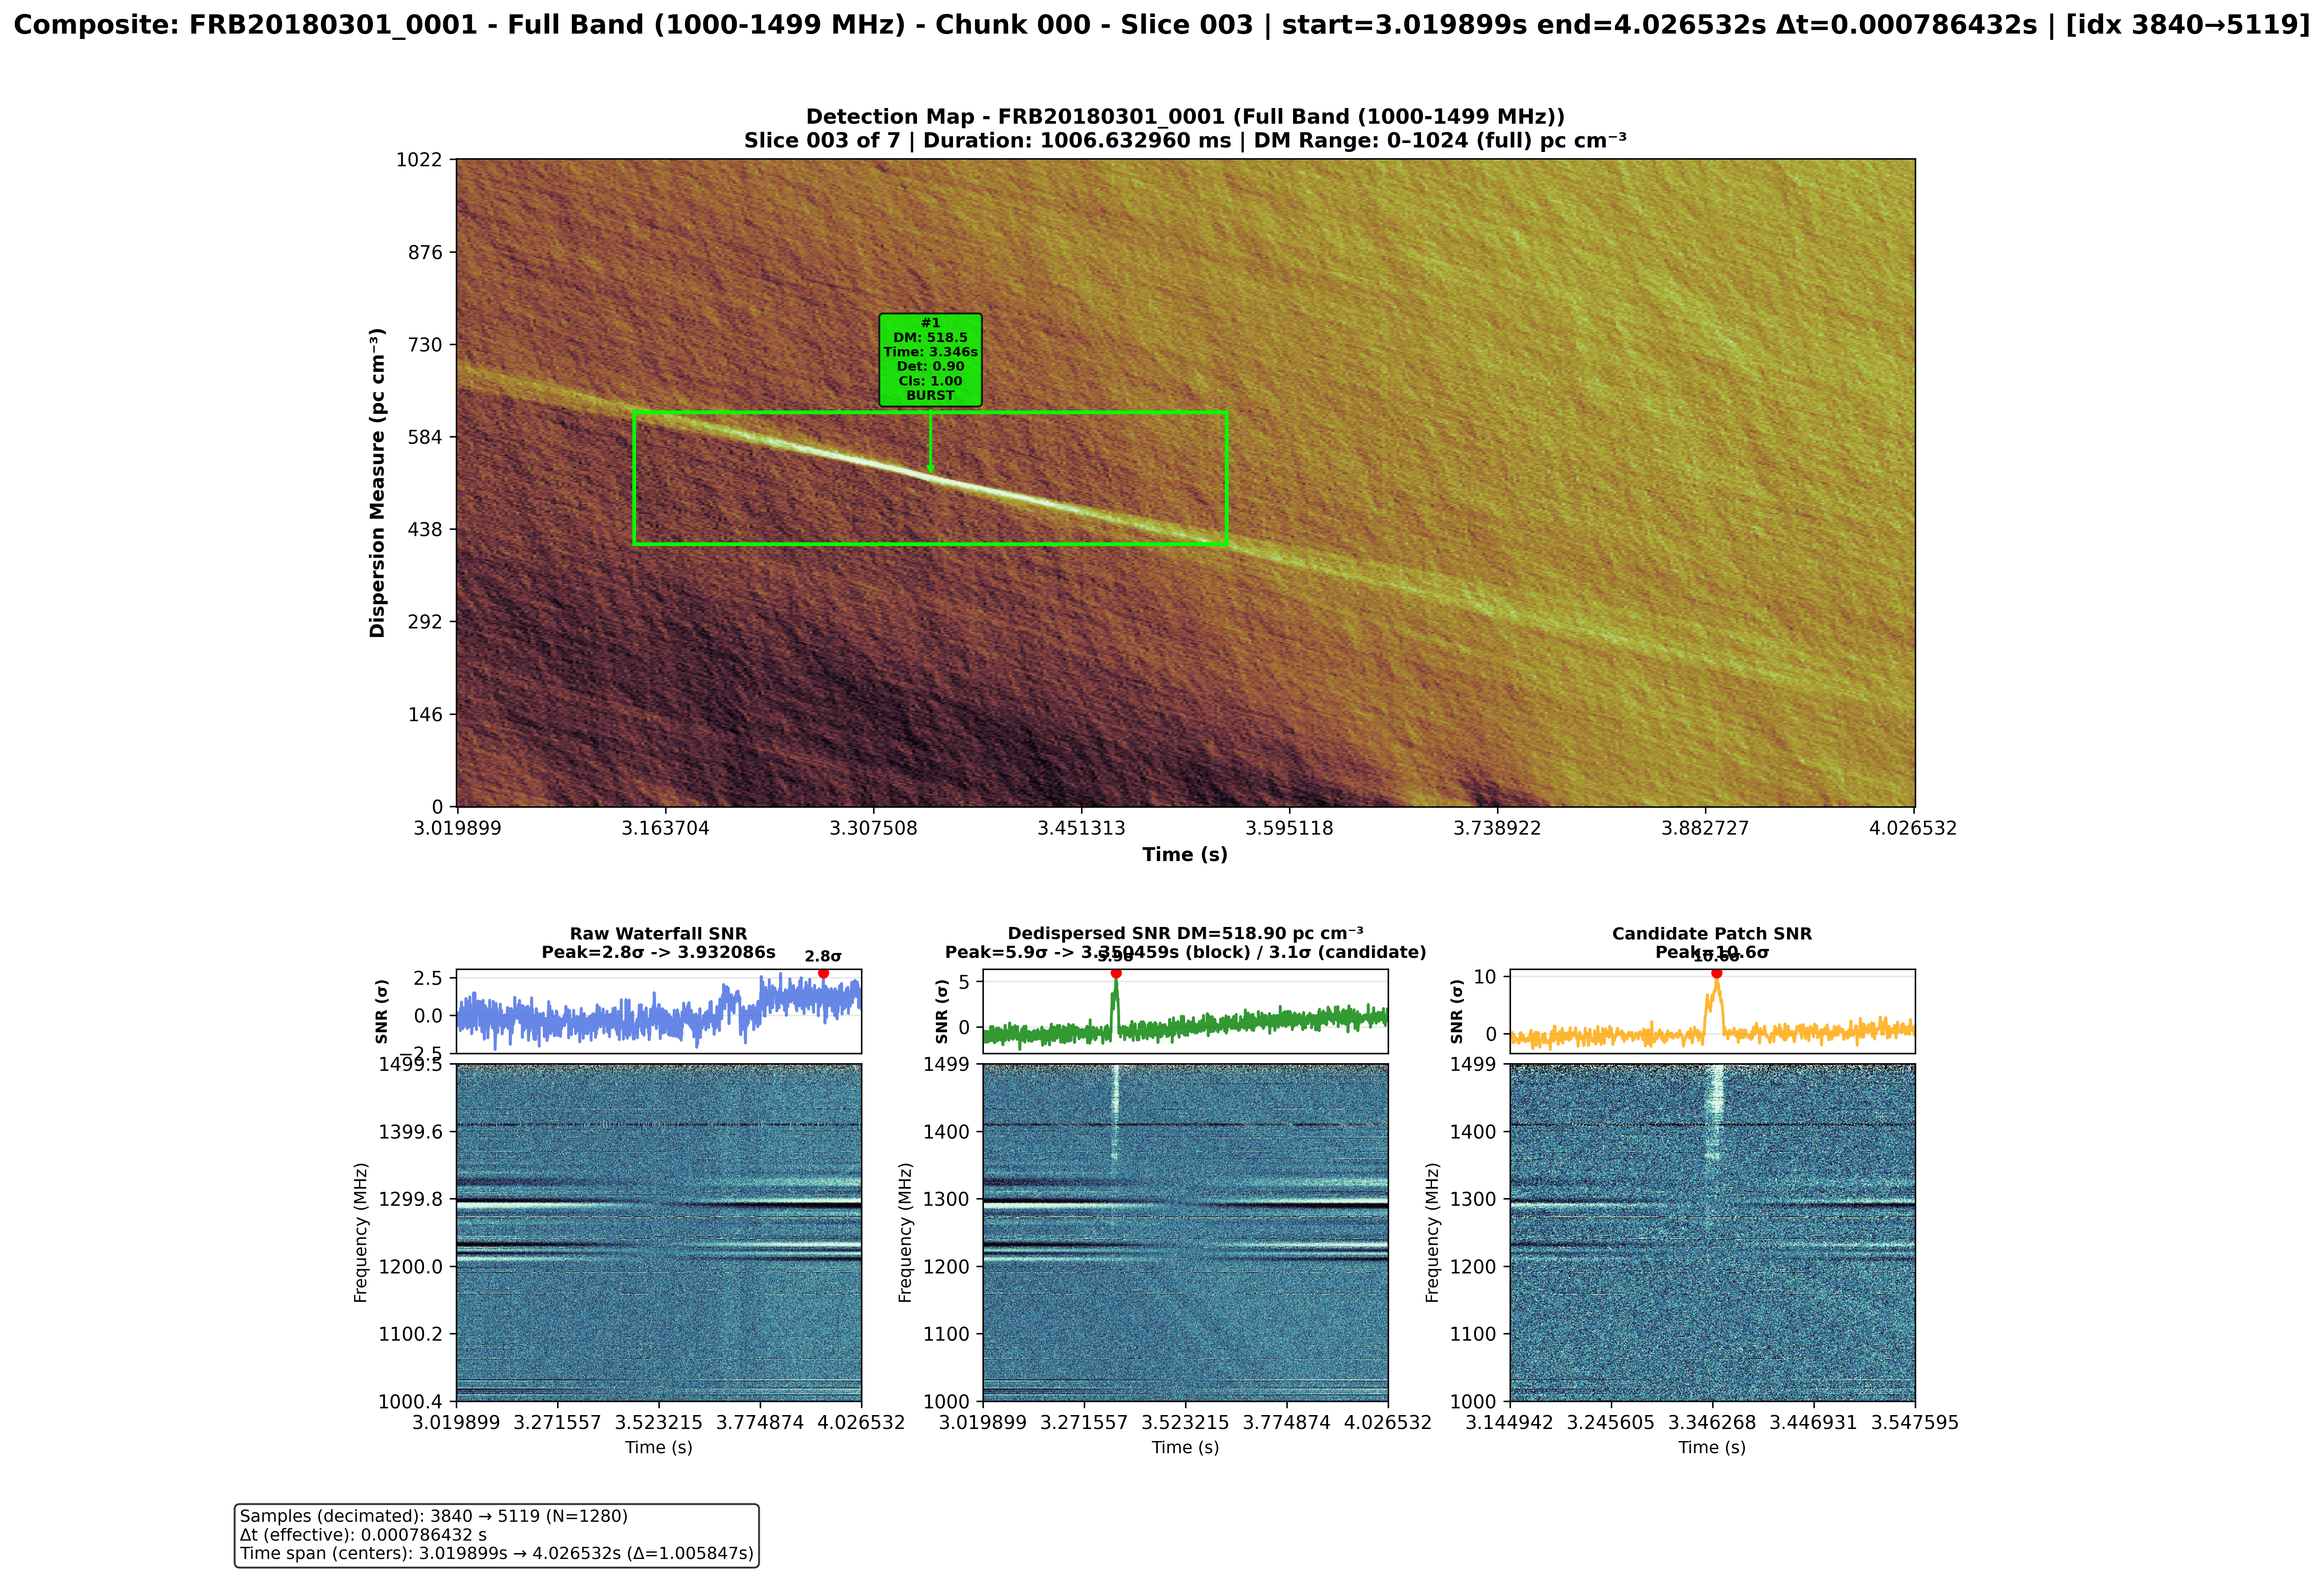
\includegraphics[width=\textwidth]{figures/FRB20180301_0001_slice003.png}
    \caption[Detección FRB (FAST-FREX)]{Detección FRB con SNR de 5.9$\sigma$ mostrando mapa DM-tiempo y perfiles SNR crudo/dedispersado.}
    \label{fig:frb20180301_0001_slice003}
\end{figure}

\begin{figure}[H]
    \centering
    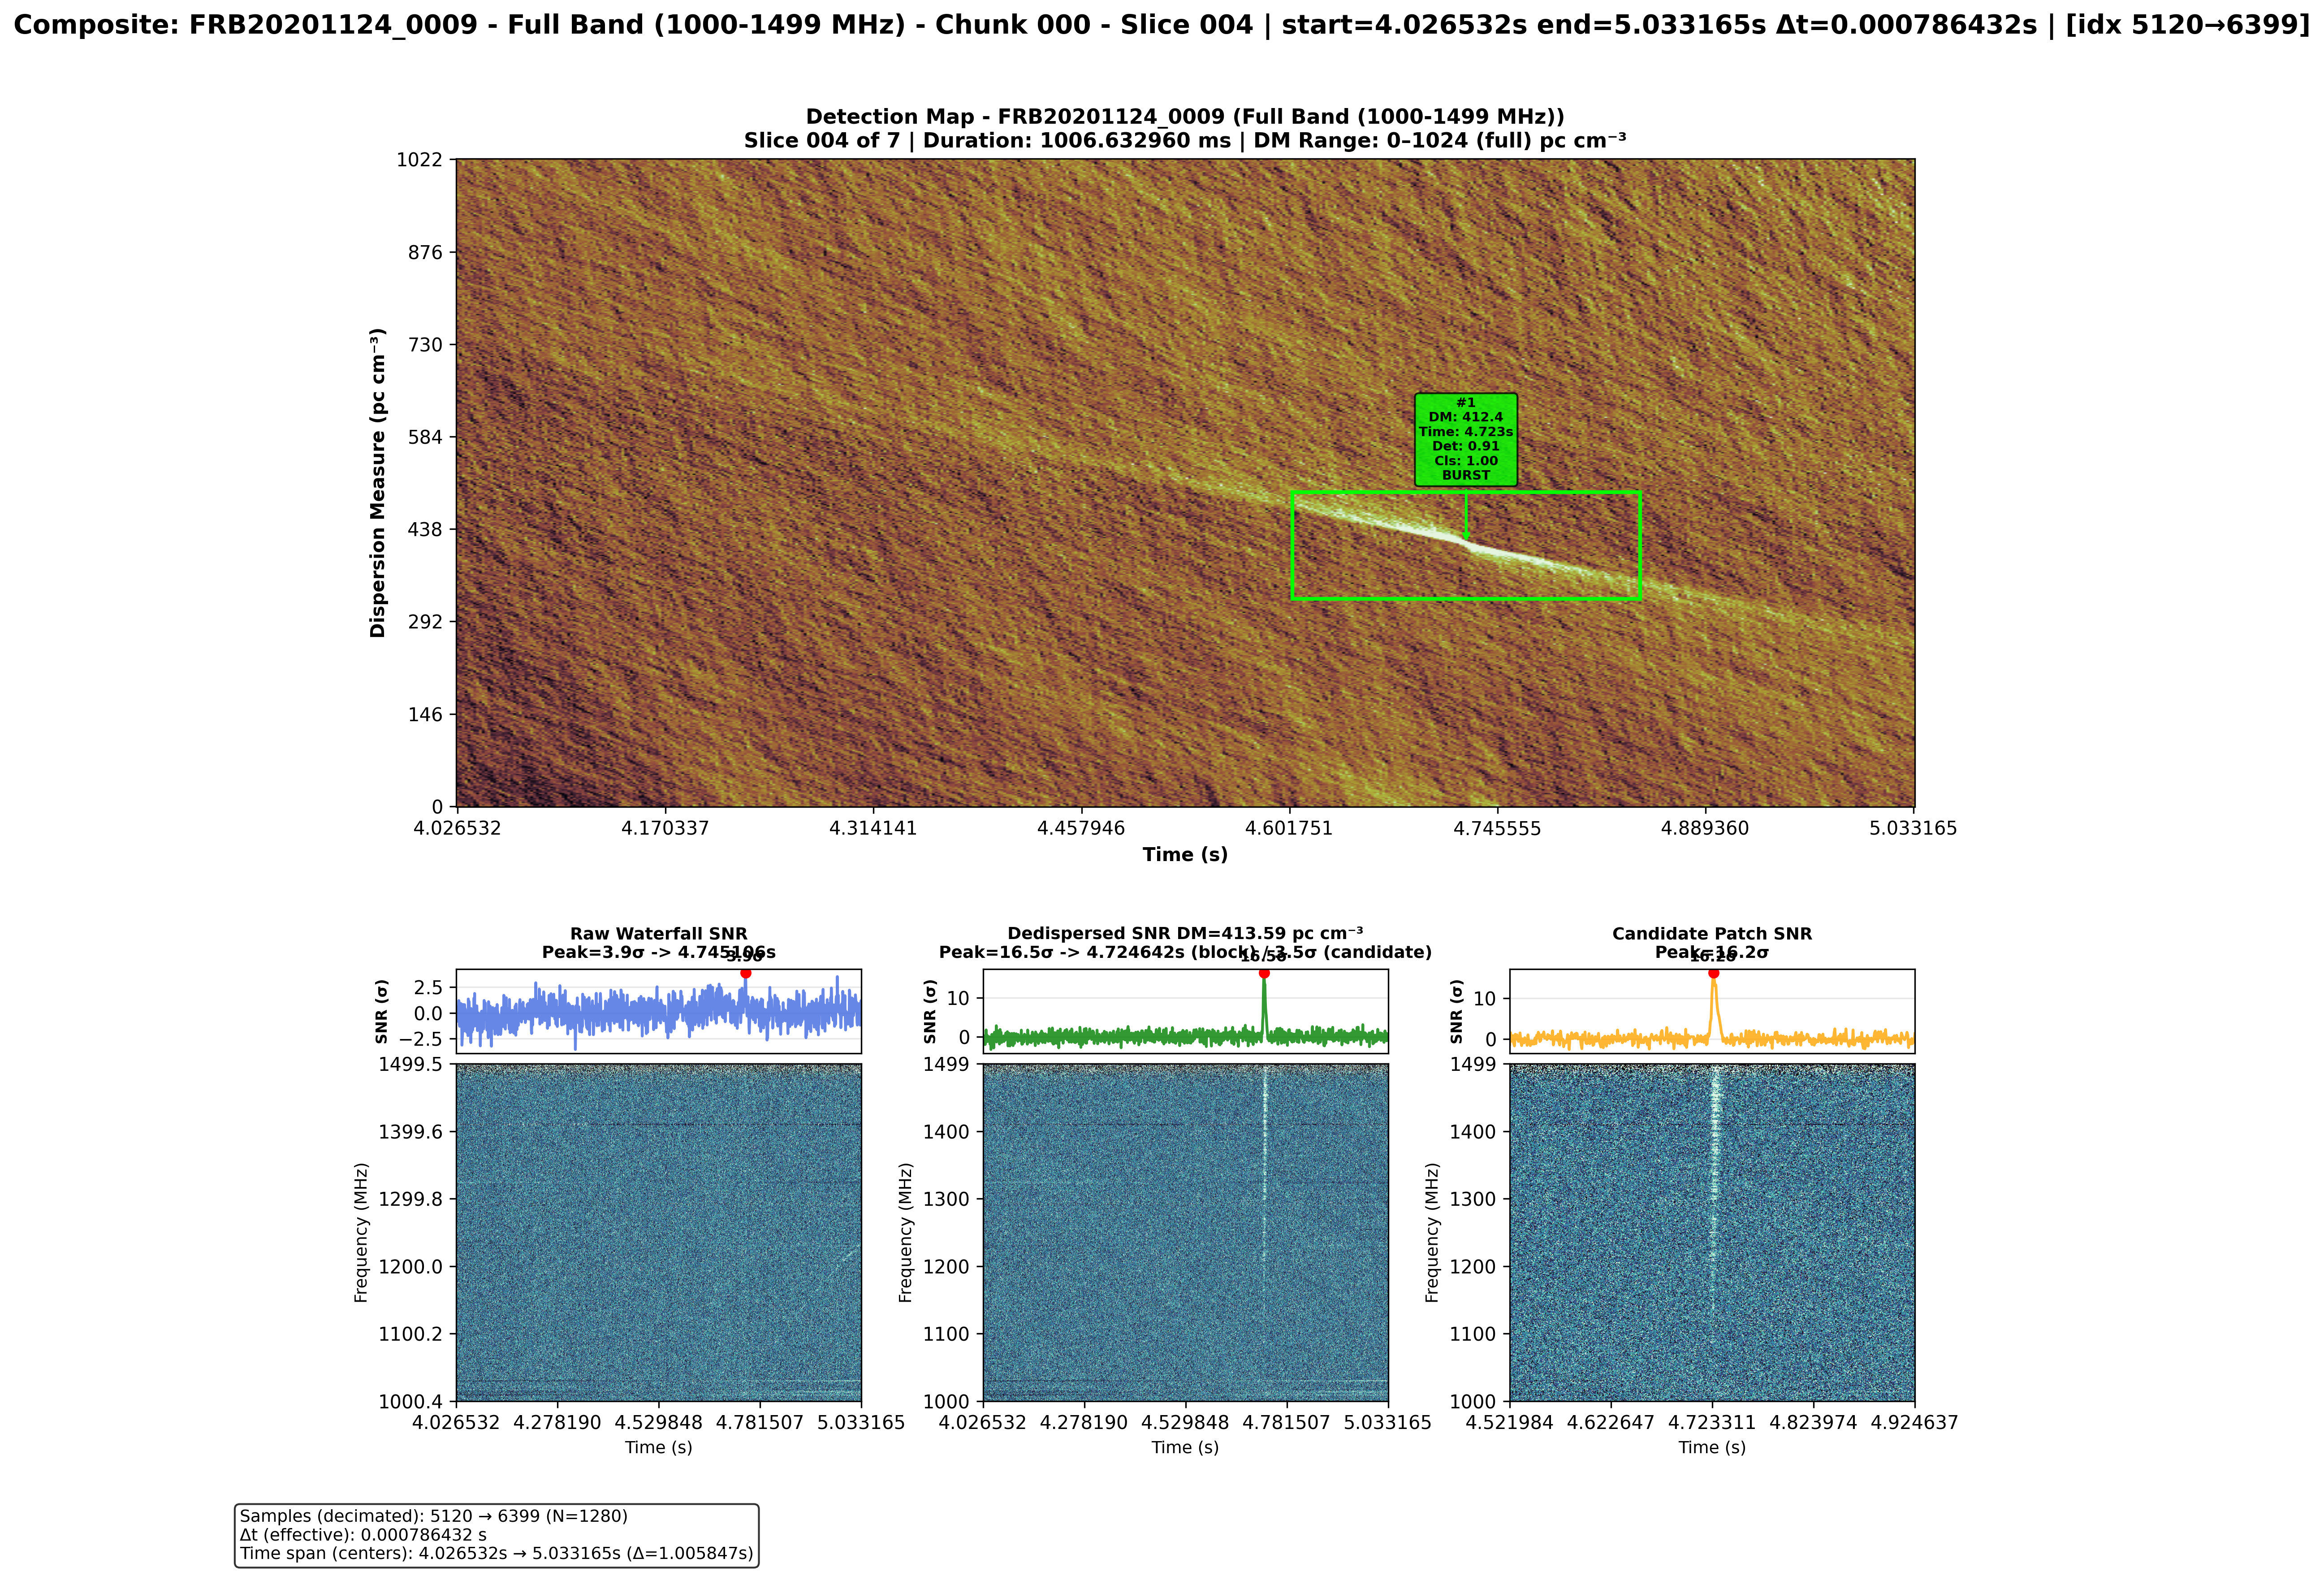
\includegraphics[width=\textwidth]{figures/FRB20201124_0009_slice004.png}
    \caption[Detección FRB adicional (FAST-FREX)]{Segundo FRB detectado con SNR de 16.5$\sigma$ confirmando efectividad del sistema.}
    \label{fig:frb20201124_0009_slice004}
\end{figure}

\subsubsection{Caso 2 - Pulsar B0355+54: Validación de Robustez Temporal y Procesamiento Secuencial}

Este caso utiliza observaciones del púlsar B0355+54 adquiridas con el radiotelescopio FAST en banda L ($\sim$1.25 GHz) en formato PSRFITS. El dataset valida mejoras de preprocesamiento: contigüidad temporal quirúrgica, streaming por slices, trazabilidad temporal precisa, manejo de discontinuidades y validación física integrada.

Características del dataset: Pulsar B0355+54\_FB\_20220918, periodo 0.156s, 117.23s duración total, 752 pulsos esperados teóricamente. Resultados: 732/752 pulsos detectados (97.3\%), 718 clasificados como BURSTS.

\begin{figure}[H]
    \centering
    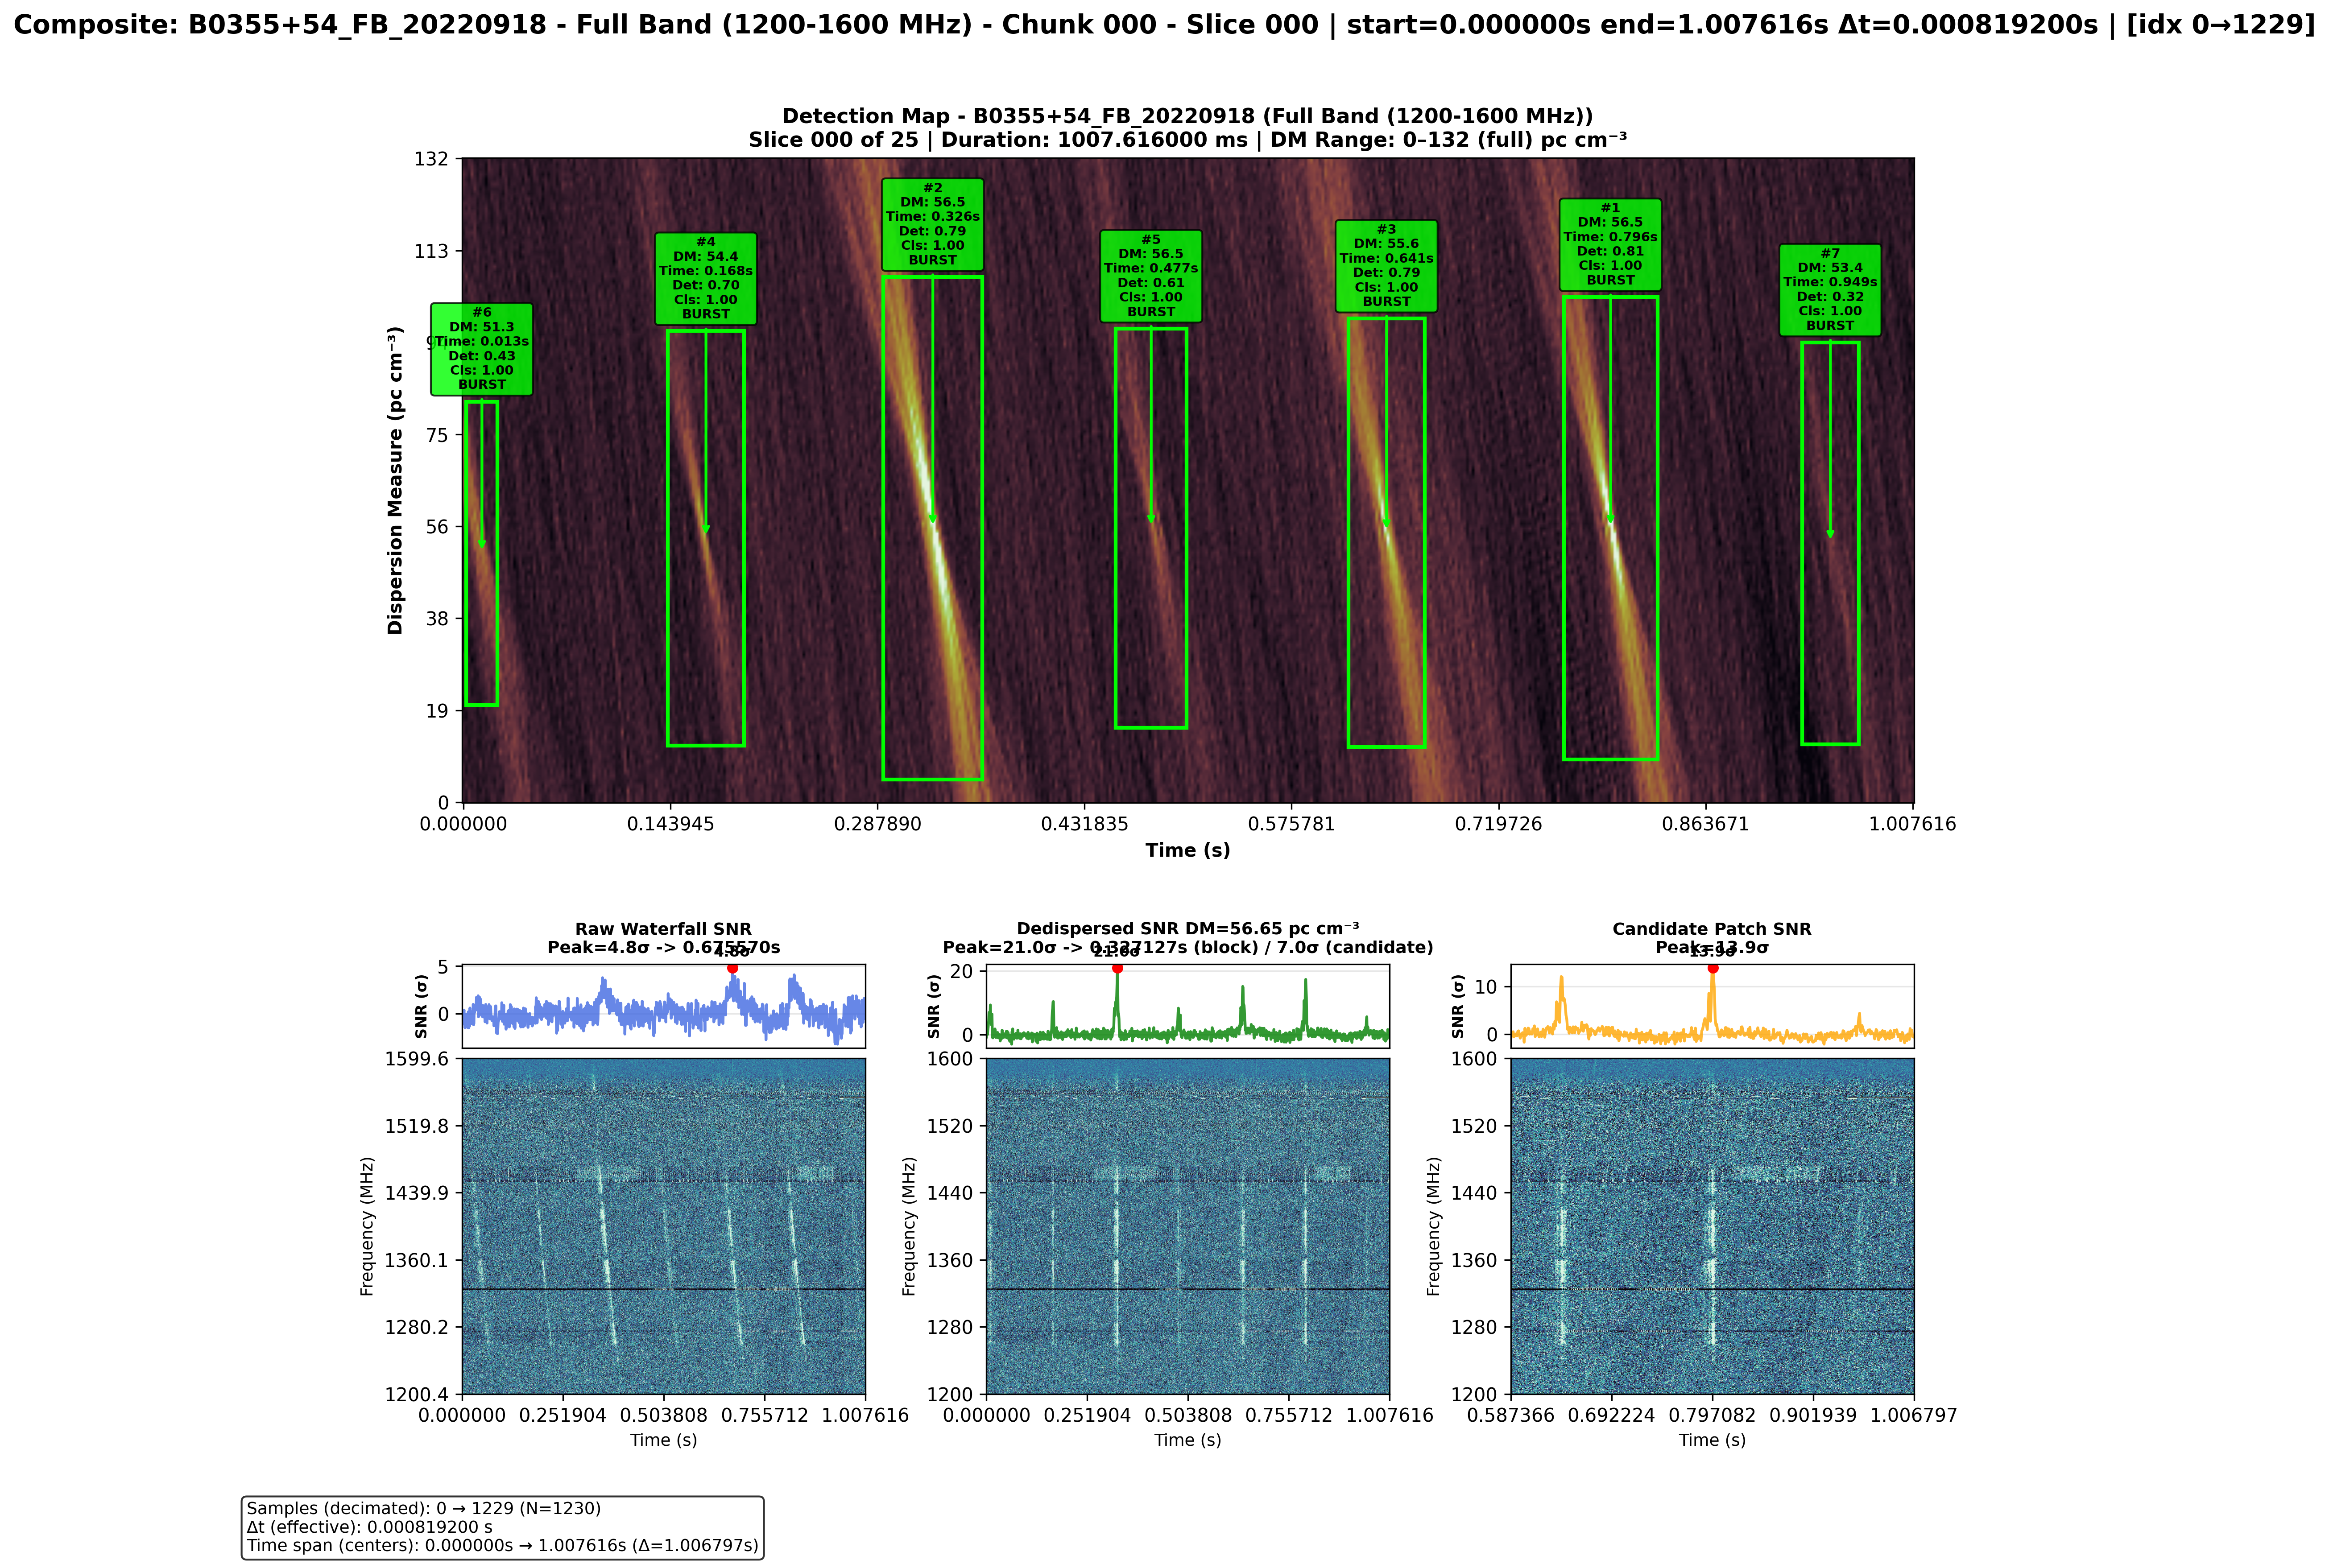
\includegraphics[width=\textwidth]{figures/B0355+54_FB_20220918_slice000.png}
    \caption[Validación continuidad temporal: Slice 000]{7 pulsos detectados en el primer segundo, todos clasificados como BURSTS (scores >0.99).}
    \label{fig:b0355_slice000}
\end{figure}


\begin{figure}[H]
    \centering
    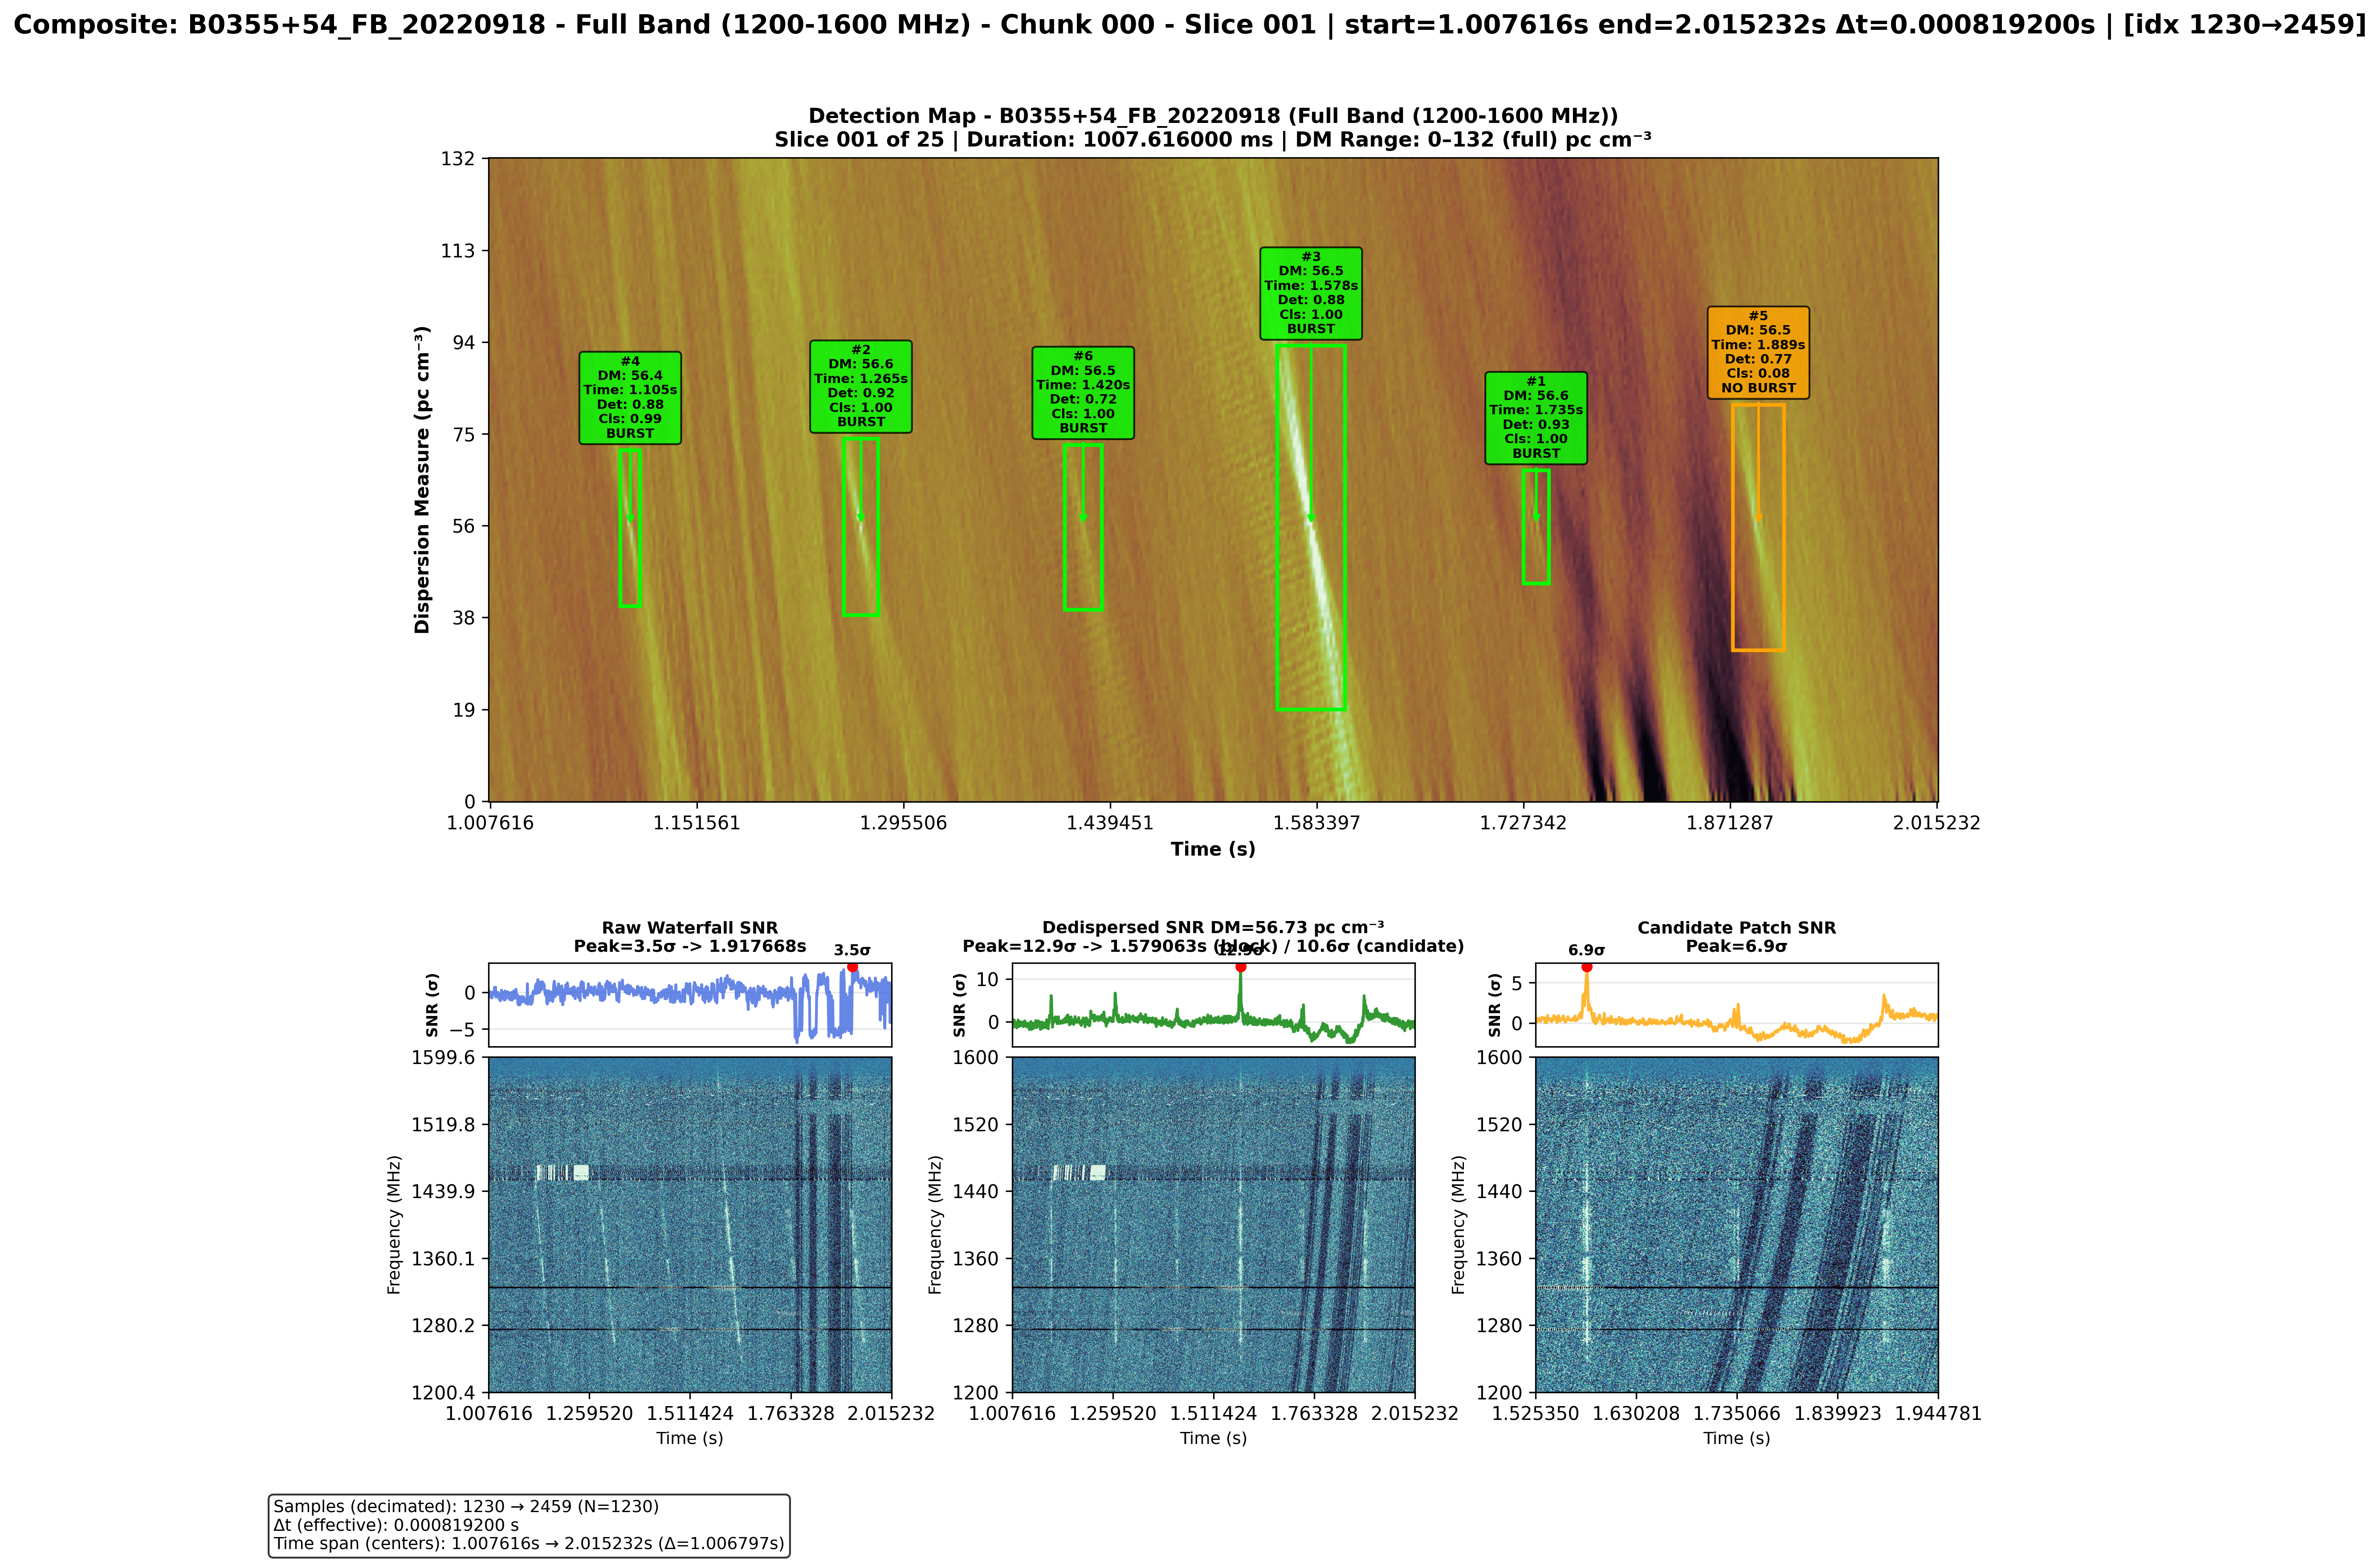
\includegraphics[width=\textwidth]{figures/B0355+54_FB_20220918_slice001.png}
    \caption[Validación continuidad temporal: Slice 001]{5 pulsos clasificados como BURSTS y 1 como NO BURST.}
    \label{fig:b0355_slice001}
\end{figure}

El resultado confirma continuidad temporal y precisión de las redes pre-entrenadas.

\begin{figure}[H]
    \centering
    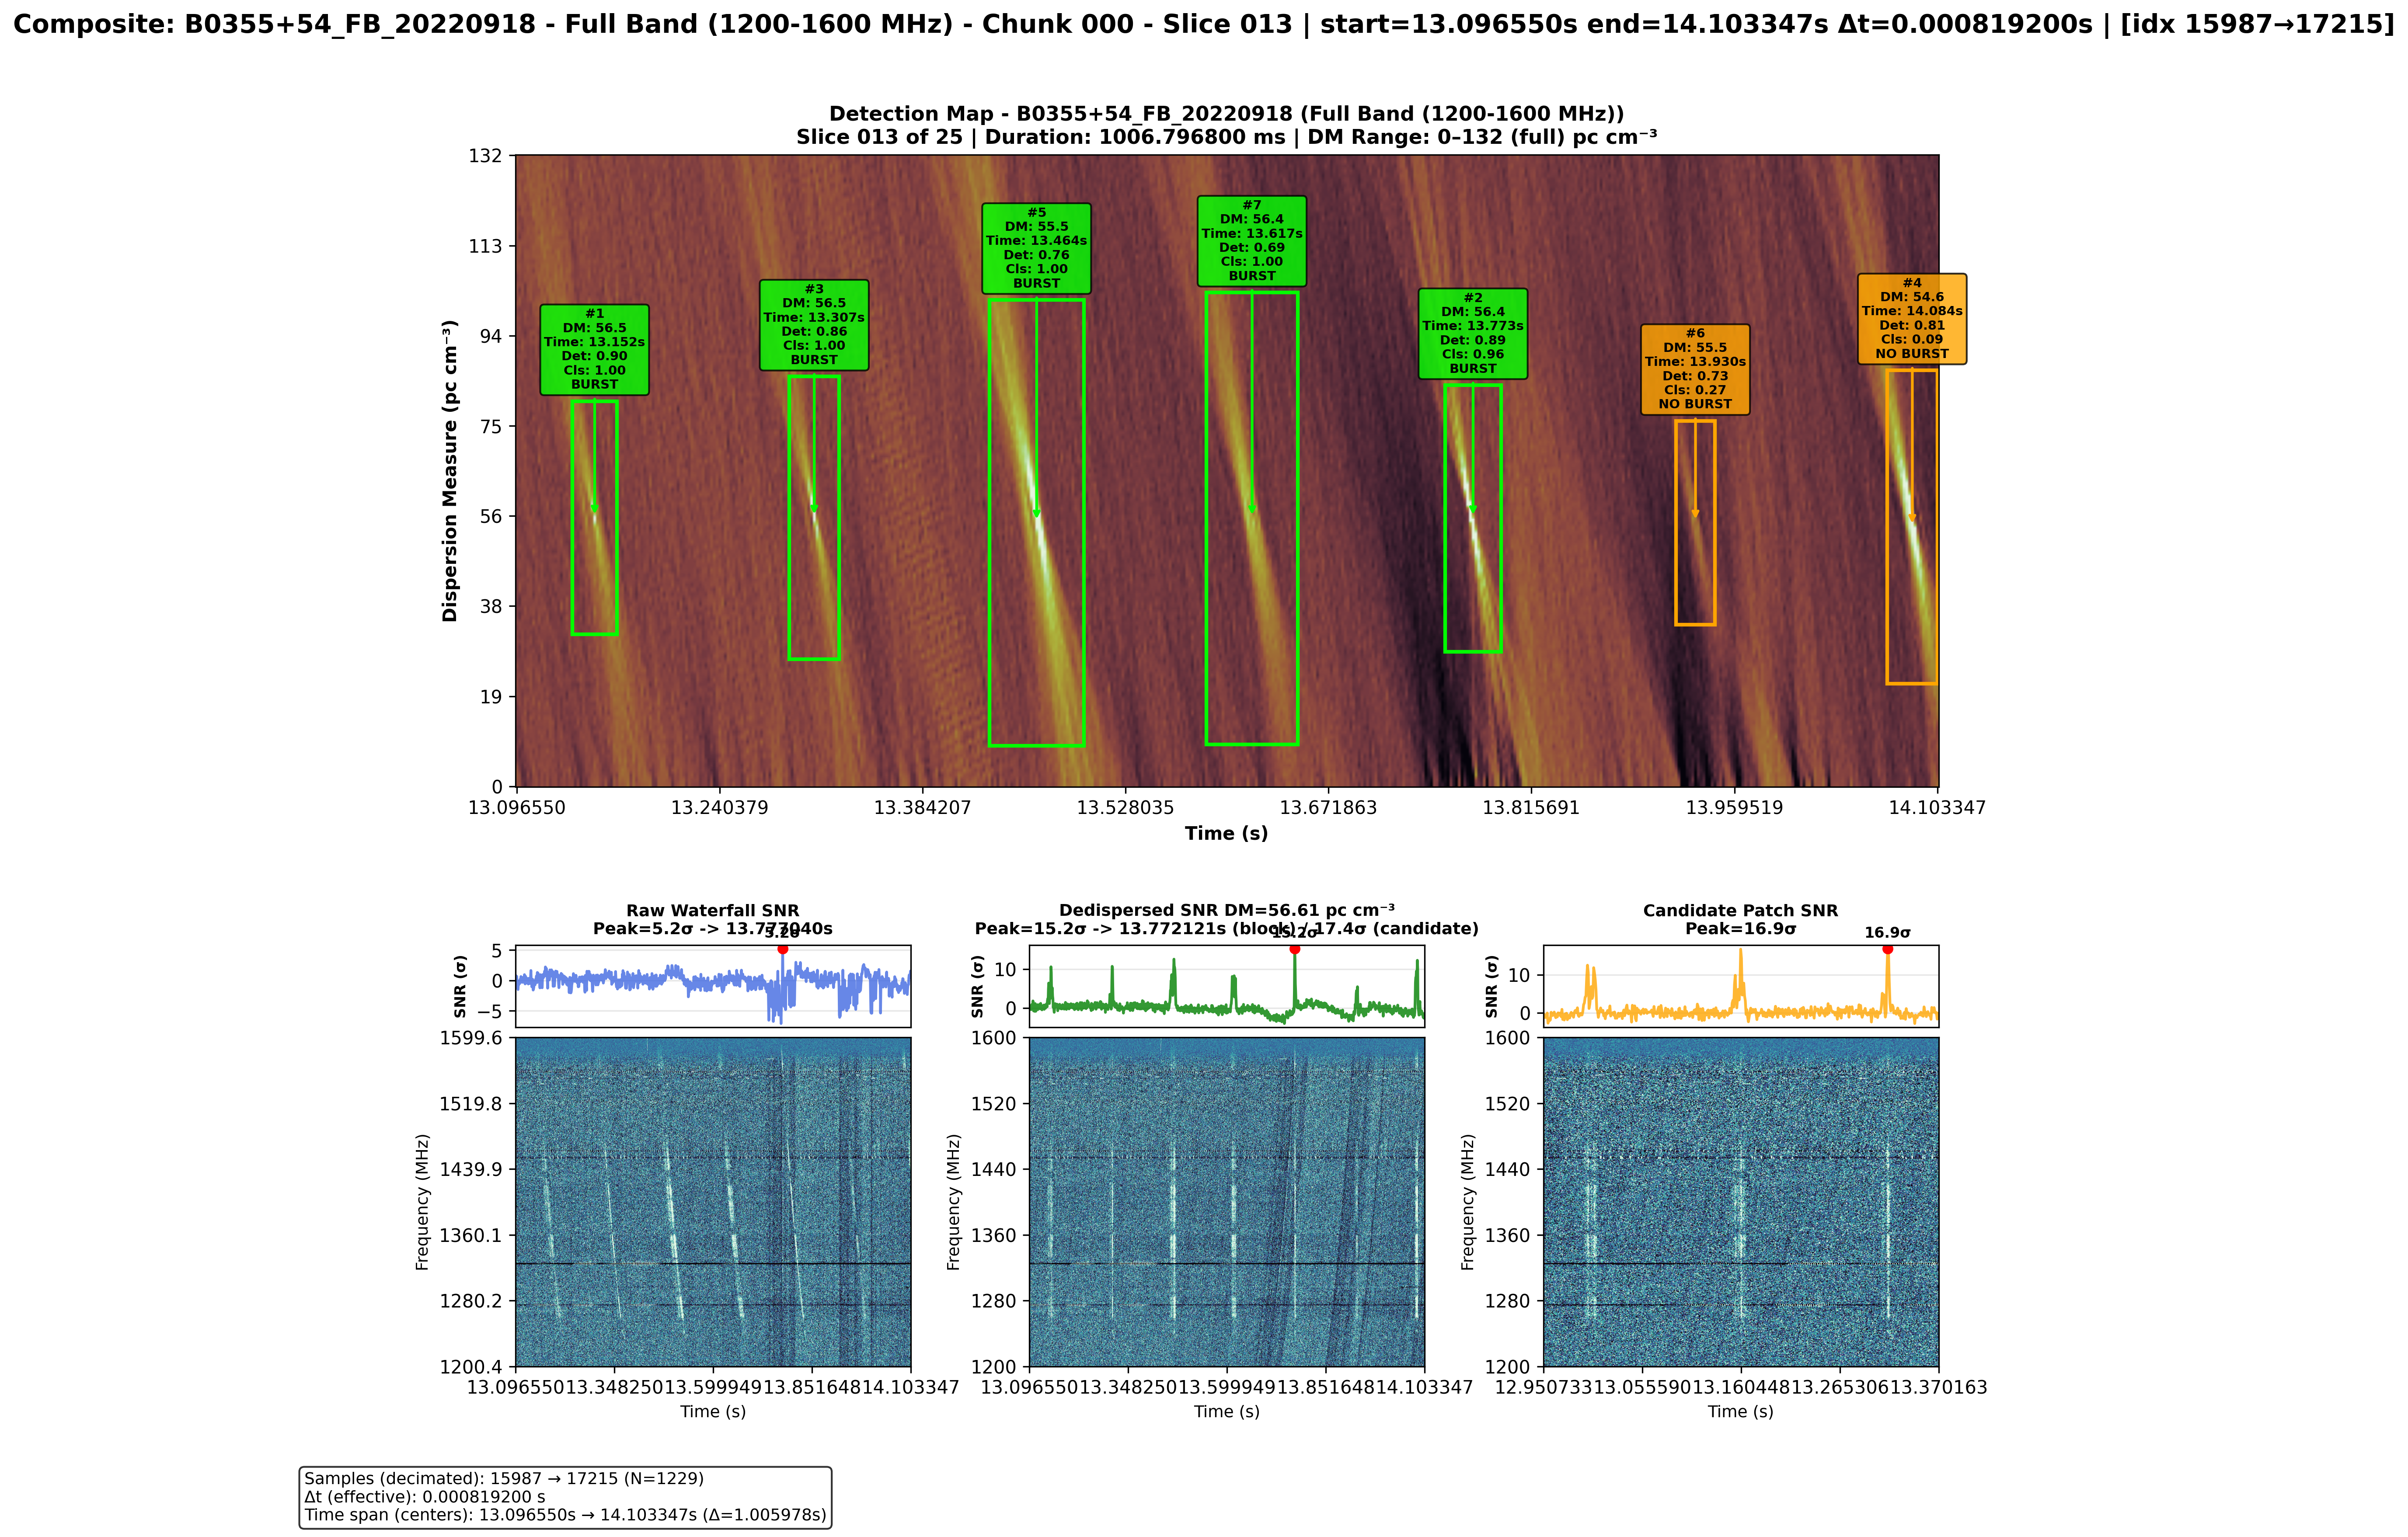
\includegraphics[width=\textwidth]{figures/B0355+54_FB_20220918_slice013.png}
    \caption[Pulso dudoso en la clasificación]{Eventos con alta detección (0.73-0.81) pero baja clasificación (0.09-0.27) clasificados como NO BURST, demostrando capacidad para señales ambiguas.}
    \label{fig:b0355_slice013}
\end{figure}

\subsubsection{Caso 3 - FRB 121102: Validación de Escalabilidad E2E y Descubrimiento Científico}

FRB 121102 valida escalabilidad E2E con archivos multi-gigabyte del radiotelescopio Effelsberg que exceden memoria disponible, forzando operación integrada: ingesta masiva, chunking con solapamiento, gestión inteligente RAM/VRAM y procesamiento E2E sin intervención manual.

Se procesaron 6 archivos observacionales del radiotelescopio Effelsberg de 100m (Alemania) en banda L ($\sim$1.4 GHz), cada uno de $\sim$4 GB en formato PSRFITS, reportados por \cite{cruces2020frb121102}, con ground truth de 24 eventos confirmados. Resultados: 41 eventos detectados, Recall=100\% (24/24 eventos conocidos recuperados), 17 candidatos nuevos identificados, 2 confirmados como genuinos (SNR 6.3$\sigma$ y 12.0$\sigma$, DM$\sim$564 pc cm$^{-3}$).

% Las detecciones completas se documentan en Anexo A: bursts confirmados por literatura (Tabla \ref{tab:anexo_confirmed_bursts}), nuevos eventos confirmados (Tabla \ref{tab:anexo_new_confirmed_bursts}), y candidatos pendientes (Tabla \ref{tab:anexo_candidate_bursts}). El histograma de distribución temporal (Figura \ref{fig:frb121102_histogram}) muestra concentración de eventos en archivos 3098 y 3100, consistente con ventanas de actividad del repetidor.

\begin{figure}[H]
    \centering
    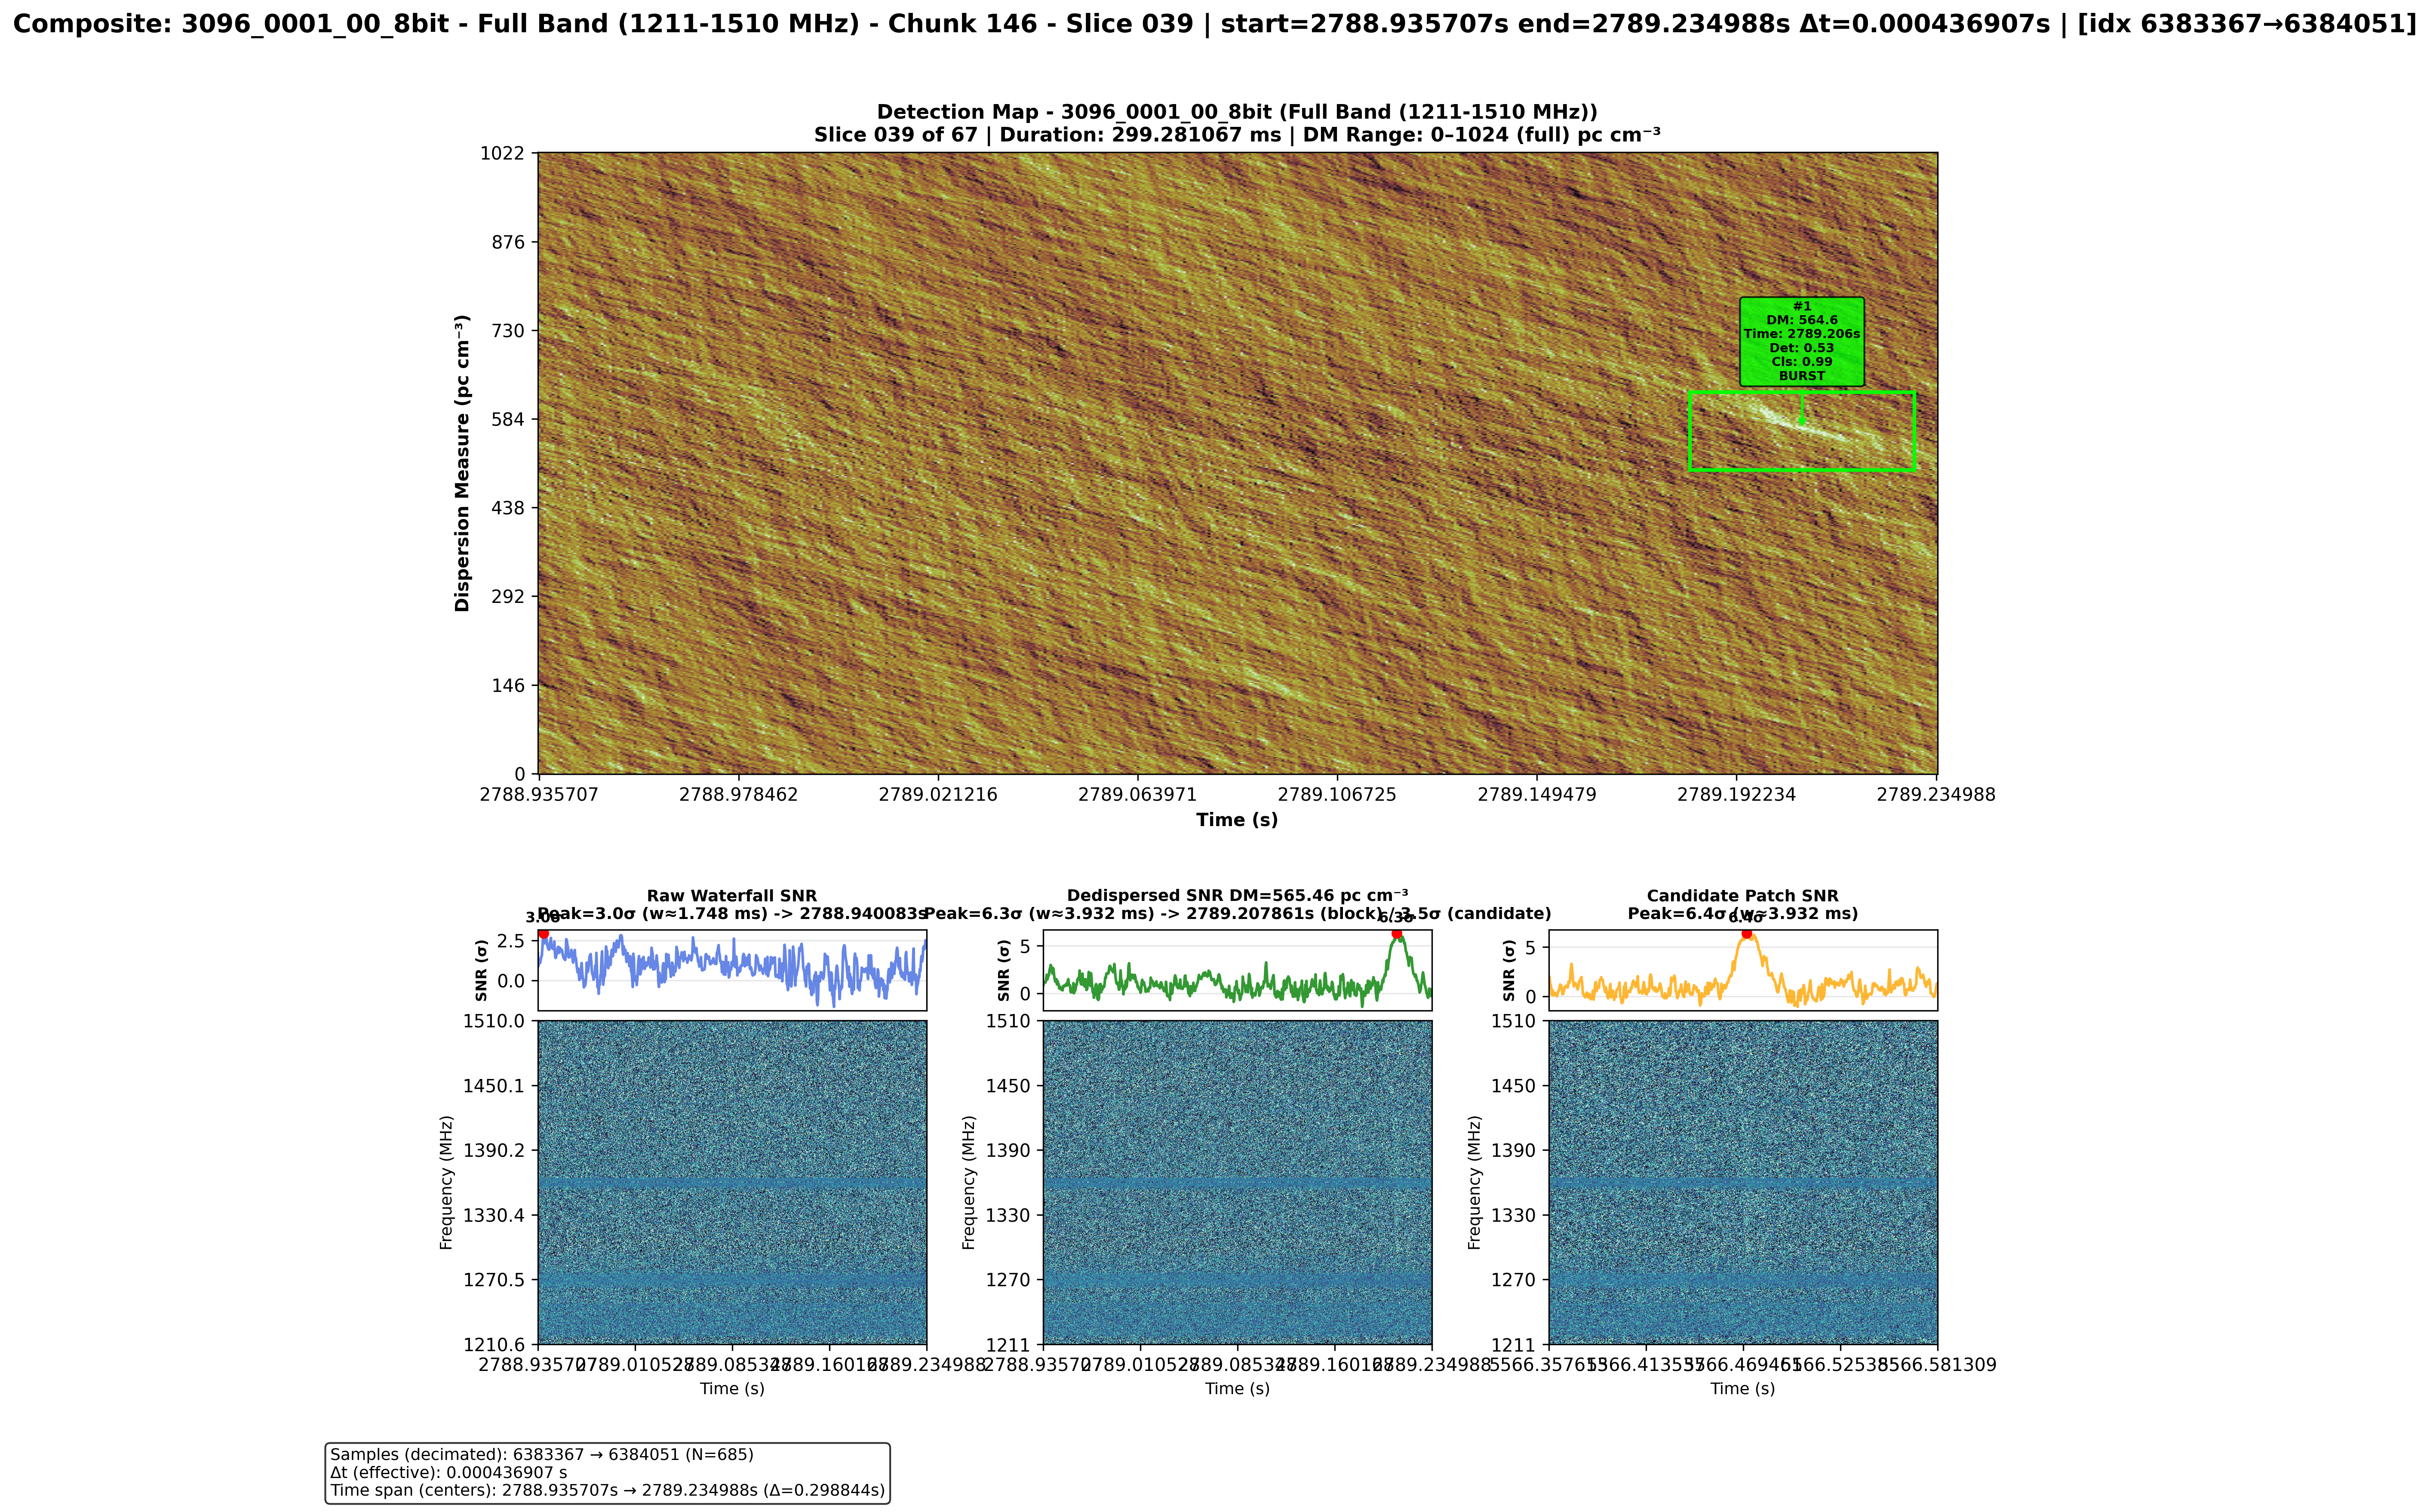
\includegraphics[width=\textwidth]{figures/3096_0001_00_8bit_slice039.png}
    \caption[FRB121102: nuevo evento confirmado (3096\_...\_slice039)]{Primer nuevo evento confirmado: DM=563.6 pc cm$^{-3}$, Time=2421.559296s, SNR=6.3$\sigma$, 100\% confirmado por astrónomos colaboradores.}
    \label{fig:new_event_3096}
\end{figure}

\begin{figure}[H]
    \centering
    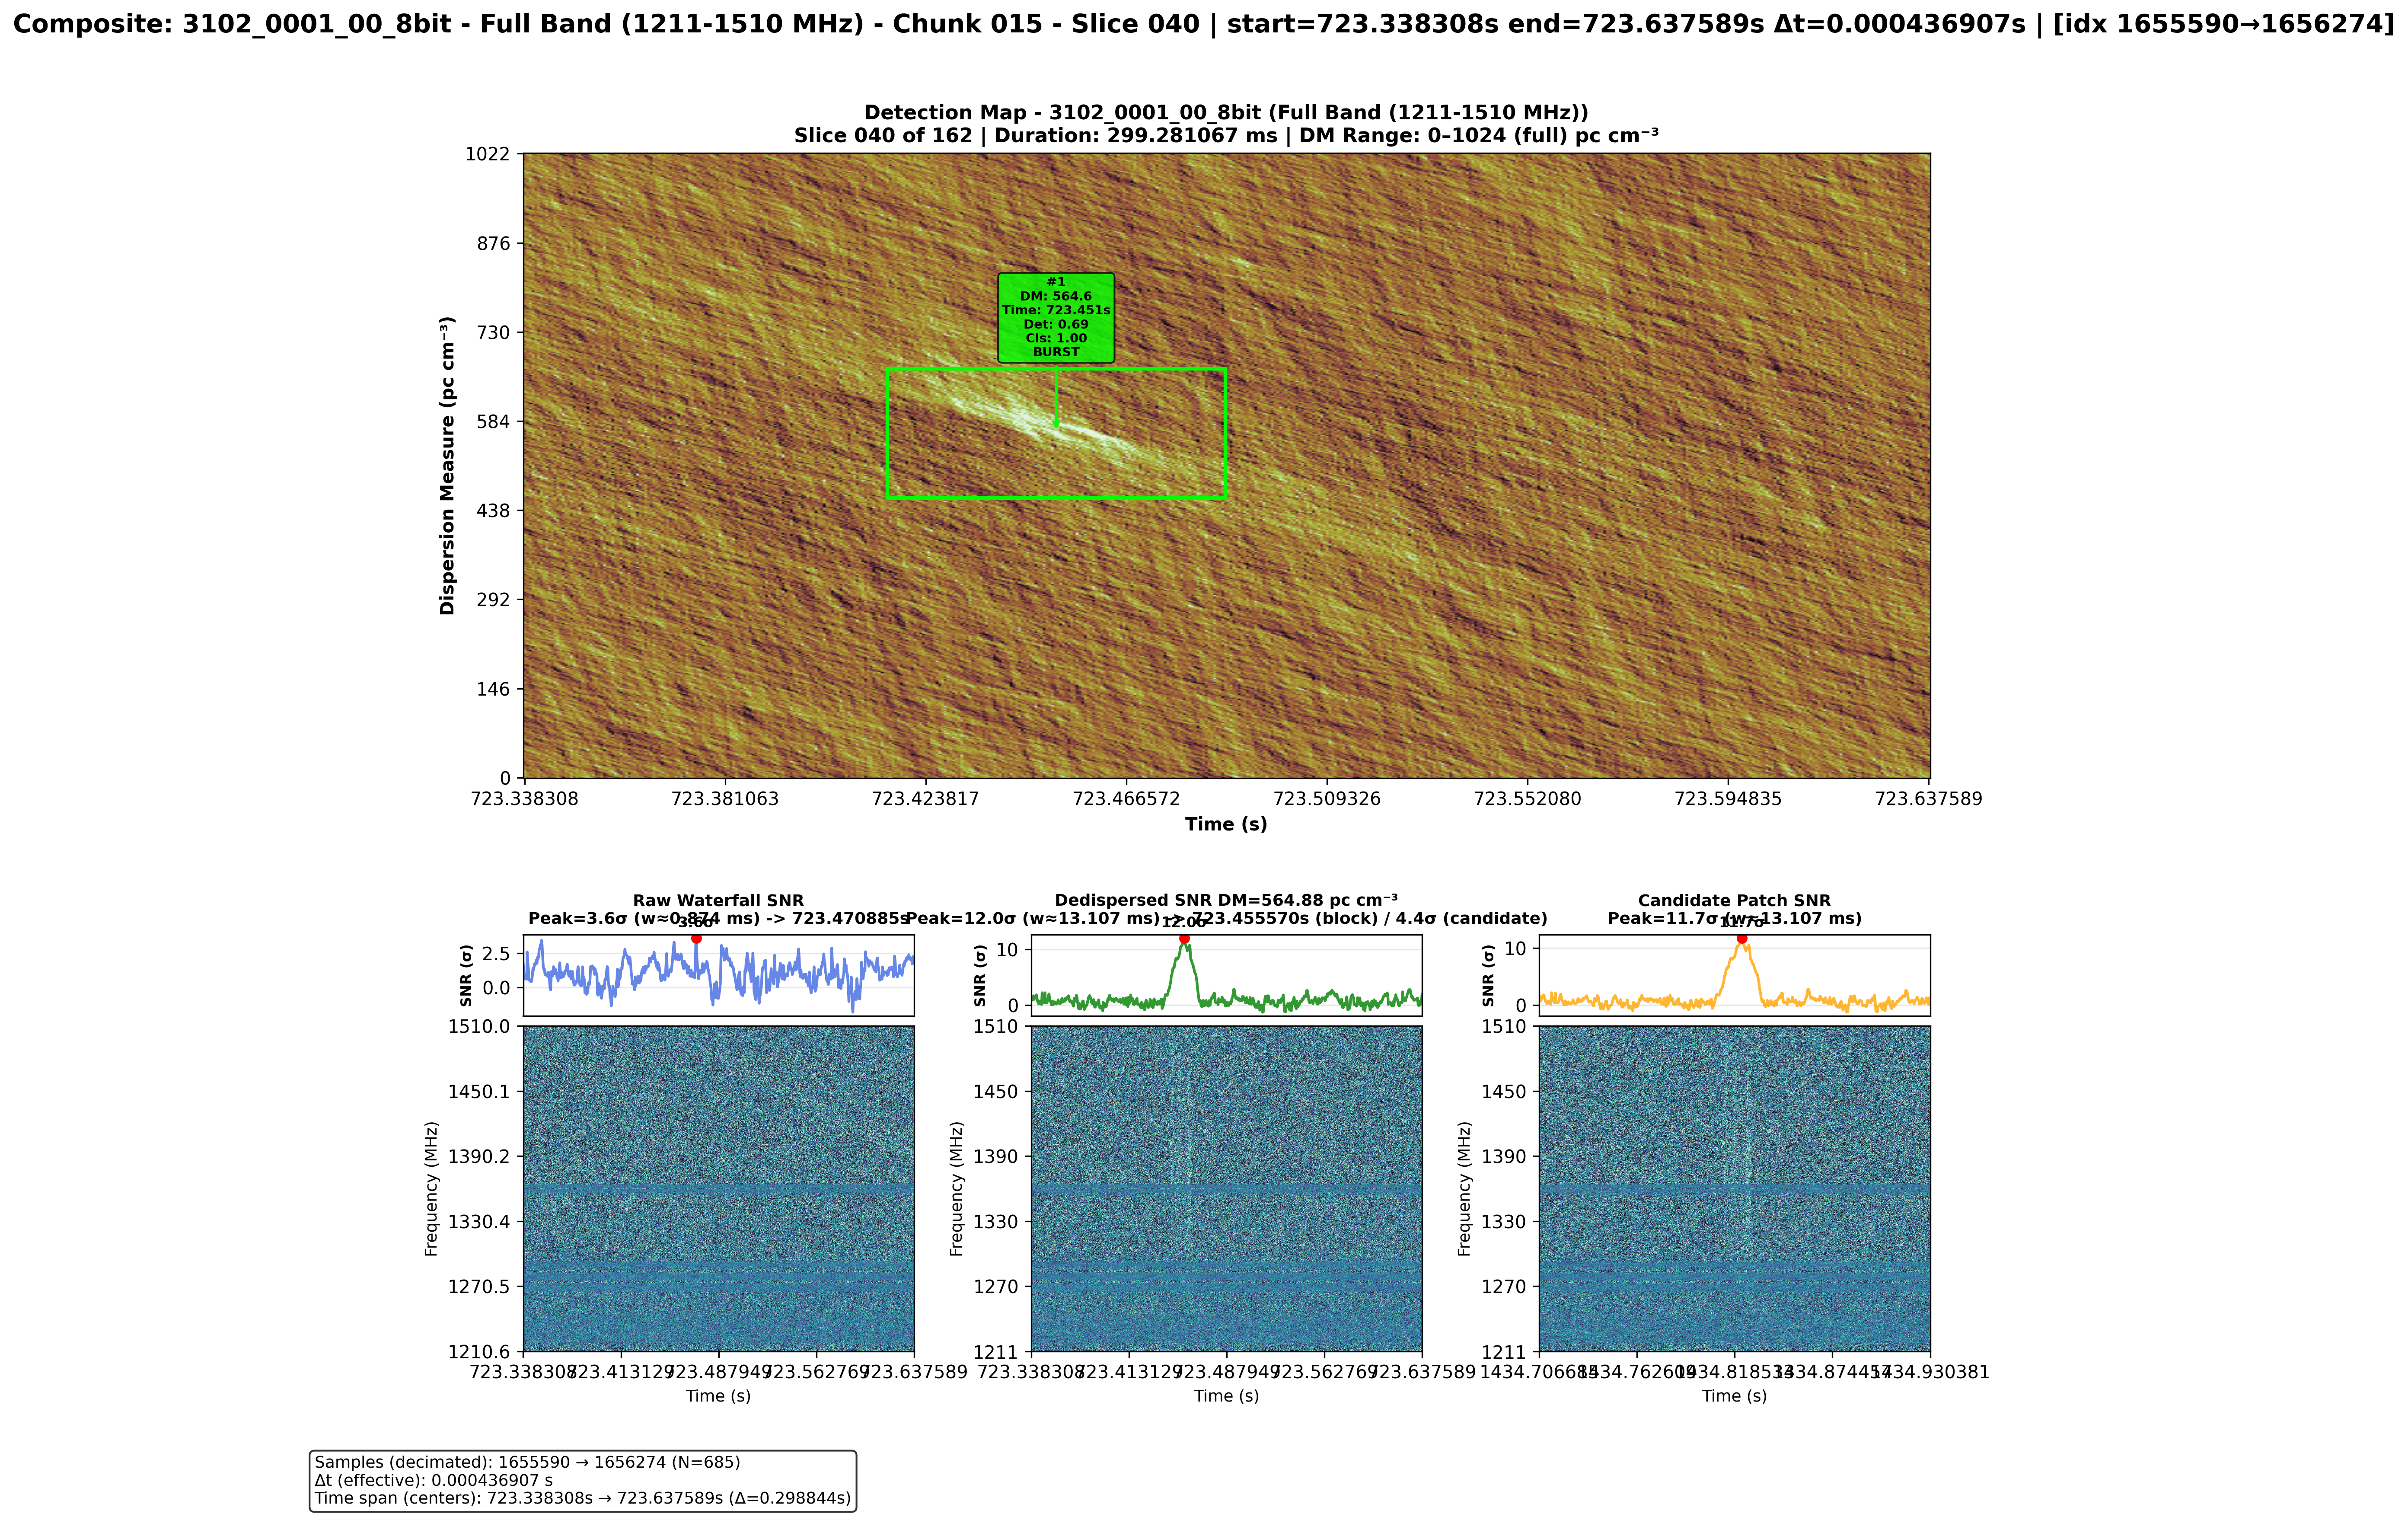
\includegraphics[width=\textwidth]{figures/3102_0001_00_8bit_slice040.png}
    \caption[FRB121102: nuevo evento confirmado (3102\_...\_slice040)]{Segundo nuevo evento confirmado: DM=564.88 pc cm$^{-3}$, Time=723.455399s, SNR=12.0$\sigma$, uno de los bursts más brillantes detectados, 100\% confirmado.}
    \label{fig:new_event_3102}
\end{figure}

% \begin{figure}[H]
%     \centering
%     \includegraphics[width=0.8\textwidth]{figures/frb121102_detection_histogram.png}
%     \caption[Histograma de detecciones FRB121102]{Distribución temporal de detecciones por archivo de observación. Morado: bursts confirmados por literatura; Celeste: nuevos candidatos sin confirmar; Verde: nuevos eventos confirmados. La concentración en archivos 3098 y 3100 es consistente con ventanas de actividad del repetidor. \textit{Fuente: Elaboración propia}.}
%     \label{fig:frb121102_histogram}
% \end{figure}

Los resultados validan integralmente el Componente 1. El pipeline procesó exitosamente archivos multi-gigabyte sin errores de memoria ni degradación de rendimiento, operando sin intervención manual desde ingesta hasta visualización. El recall perfecto (26/26 eventos detectados: 24 de literatura + 2 nuevos confirmados) demuestra que el sistema de chunking con solapamiento controlado no introduce puntos ciegos temporales, validando la continuidad temporal quirúrgica implementada. El descubrimiento de 2 nuevos bursts confirmados demuestra capacidad de descubrimiento científico genuino.

\subsection{VALIDACIÓN DEL COMPONENTE 2: DRAFTS++ - Extensión a Alta Frecuencia - Cuatro Líneas de Investigación}

La validación del Componente 2 examina la efectividad de DRAFTS++ en el régimen milimétrico (86 GHz), donde la firma dispersiva tradicional se comprime significativamente debido a la dependencia $\Delta t_{\mathrm{ms}} \propto \nu^{-2}$. En este régimen, el patrón bow-tie característico de FRBs en bajas frecuencias (1.4 GHz) colapsa, desafiando a detectores entrenados en firmas dispersivas desarrolladas.

Para todas las líneas de investigación se validó utilizando observaciones del Atacama Large Millimeter/submillimeter Array (ALMA, Chile) en modo \emph{phased array}, específicamente datos del magnetar del Centro Galáctico PSR J1745-2900 observados en Banda 3 ($\sim$86 GHz, ancho de banda 2 GHz) durante campañas de 2017, proporcionadas por \cite{veracasanova2025}. Este dataset constituye ground truth mediante 8 pulsos confirmados independientemente con PRESTO (Tabla~\ref{tab:veracasanova_reference}), permitiendo evaluación objetiva de cada estrategia. Los datos fueron adquiridos con resolución temporal de $\sim$8 $\mu$s y formato PSRFITS.

\begin{table}[H]
    \centering
\caption{Ground truth: Pulsos del magnetar PSR J1745-2900 reportados por Vera-Casanova et al. (2025), utilizados para validación de todas las líneas de investigación.}
    \label{tab:veracasanova_reference}
\small
    \begin{tabular}{|c|c|}
        \hline
\textbf{File} & \textbf{Timestamp (s)} \\
        \hline
        142\_0003 & 39.977 \\
142\_0006 & 10.882, 25.829 \\
        153\_0006 & 23.444 \\
230\_0002 & 2.3, 17.395 \\
        230\_0003 & 36.548 \\
        242\_0005 & 44.919 \\
        \hline
\multicolumn{2}{|c|}{Total: 8 pulsos confirmados} \\
\hline
    \end{tabular}
\end{table}

Las métricas de evaluación son estándar: Recall, que mide sensibilidad (fracción de pulsos genuinos detectados), Precision, que cuantifica especificidad (proporción de detecciones correctas), y F1-score que sintetiza el balance entre ambas. Los resultados se complementan con análisis de casos representativos que ilustran modos de éxito y falla de cada estrategia.

\subsubsection{Línea 1: Validación de Transferibilidad del Pipeline Clásico mediante Adaptación Paramétrica}

Esta línea establece el baseline de rendimiento del pipeline clásico (CenterNet + ResNet18) en alta frecuencia sin modificaciones arquitecturales, evaluando si ajustes paramétricos simples pueden compensar la compresión del bow-tie. El experimento compara dos configuraciones de umbral de detección: conservadora (DET\_PROB = 0.3, optimizada en bajas frecuencias) y sensible (DET\_PROB = 0.05, factor x6 más permisivo), aislando el efecto del umbral sobre sensibilidad y especificidad.

Los resultados revelaron comportamiento bimodal dramático. Con el umbral estándar (DET\_PROB = 0.3), el sistema falló completamente: ninguno de los 8 pulsos de referencia fue detectado. Este resultado confirma que modelos optimizados para bow-ties desarrollados no transfieren directamente a regímenes comprimidos, independientemente de la calidad del entrenamiento original.

Al reducir el umbral en factor x6 (DET\_PROB = 0.05), el sistema recuperó sensibilidad parcial detectando 7/8 pulsos (Recall = 87.5\%), pero introdujo aproximadamente 12 candidatos espurios, degradando la precisión a 36.8\%. El F1-score de 51.8\% refleja el trade-off fundamental entre sensibilidad y especificidad inherente a la adaptación paramétrica: ajustar el umbral desplaza el punto de operación en la curva ROC pero no expande el dominio de representación del modelo. La Tabla \ref{tab:comparacion_umbrales_linea1} sintetiza estas métricas.

\begin{table}[H]
    \centering
    \caption{Rendimiento del pipeline clásico adaptado según configuración de umbral. Las métricas cuantifican el trade-off fundamental entre sensibilidad (recall) y especificidad (precision) en adaptación paramétrica para alta frecuencia. \textit{Fuente: Elaboración propia}.}
    \label{tab:comparacion_umbrales_linea1}
    \begin{tabular}{|l|c|c|}
        \hline
        \textbf{Métrica} & \textbf{Conservadora} & \textbf{Sensible} \\
         & \textbf{(DET\_PROB = 0.3)} & \textbf{(DET\_PROB = 0.05)} \\
        \hline
        Recall & 0\% (0/8) & 87.5\% (7/8) \\
        \hline
        Precision & Indefinida & 36.8\% (7/19) \\
        \hline
        F1-Score & Indefinida & 51.8\% \\
        \hline
        Falsos Positivos & 0 & ~12 (estimado) \\
        \hline
        Caracterización & Específico/Insensible & Sensible/Impreciso \\
        \hline
    \end{tabular}
\end{table}

Dos casos ilustran el espectro de comportamientos observados. El primer pulso (Archivo 142\_0003, t=39.977s) no fue detectado con umbral conservador (Figura \ref{fig:142_0003_slice133_highProb}), pero apareció con probabilidad marginal 9\% al reducir el umbral (Figura \ref{fig:142_0003_slice133_lowProb}). Este éxito parcial sugiere que el modelo captura características relevantes de alta frecuencia, aunque requiere umbral permisivo para activarse. El costo es evidente: candidatos espurios adicionales emergen simultáneamente, introduciendo ruido de clasificación.

El segundo caso (Archivo 242\_0005, t=44.169s) permaneció indetectable en ambas configuraciones (Figuras \ref{fig:242_0005_slice149_highProb} y \ref{fig:242_0005_slice149_lowProb}). Esta falla persistente revela limitaciones arquitecturales irreductibles: ciertas señales de alta frecuencia escapan completamente al dominio de representación aprendido por el modelo, independientemente de ajustes paramétricos.

\begin{figure}[H]
    \centering
    \includegraphics[width=0.9\textwidth]{figures/2017-04-03-08-16-13_142_0003_t39.977_slice133.png}
    \caption[Caso A: Configuración conservadora]{Caso A con configuración conservadora (DET\_PROB = 0.3). El mapa de detección DM-tiempo muestra ausencia total de candidatos para el pulso confirmado en t=39.977s. El umbral estándar optimizado para bajas frecuencias resulta incompatible con características espectrales de alta frecuencia. \textit{Fuente: Elaboración propia}.}
    \label{fig:142_0003_slice133_highProb}
\end{figure}

\begin{figure}[H]
    \centering
    \includegraphics[width=0.9\textwidth]{figures/2017-04-03-08-16-13_142_0003_t39.977_slice133-lowProb.png}
    \caption[Caso A: Configuración sensible]{Caso A con configuración sensible (DET\_PROB = 0.05). El sistema detecta el pulso genuino en t=39.976s con probabilidad marginal 9\%, junto con candidatos espurios adicionales. La recuperación de detección mediante reducción de umbral demuestra sensibilidad paramétrica, pero a costa de especificidad reducida. \textit{Fuente: Elaboración propia}.}
    \label{fig:142_0003_slice133_lowProb}
\end{figure}

\begin{figure}[H]
    \centering
    \includegraphics[width=0.9\textwidth]{figures/2017-04-03-13_38_31_242_0005_t44.169_slice149.png}
    \caption[Caso B: Configuración conservadora]{Caso B con configuración conservadora (DET\_PROB = 0.3). Ausencia total de detecciones para pulso confirmado en t=44.169s, consistente con falla sistemática observada en configuración estándar. \textit{Fuente: Elaboración propia}.}
    \label{fig:242_0005_slice149_highProb}
\end{figure}

\begin{figure}[H]
    \centering
    \includegraphics[width=0.9\textwidth]{figures/2017-04-03-13_38_31_242_0005_t44.169_slice149-lowProb.png}
    \caption[Caso B: Configuración sensible]{Caso B con configuración sensible (DET\_PROB = 0.05). A pesar del umbral extremadamente permisivo, el pulso confirmado permanece indetectable. Esta falla persistente evidencia limitaciones arquitecturales fundamentales: ciertas características espectrales de alta frecuencia escapan al dominio de aplicación del modelo pre-entrenado, independientemente de ajustes paramétricos. \textit{Fuente: Elaboración propia}.}
    \label{fig:242_0005_slice149_lowProb}
\end{figure}
Los resultados establecen el límite superior del pipeline clásico en alta frecuencia: Recall máximo 87.5\% con Precision 36.8\%. El umbral estándar (0\% recall) resulta completamente inadecuado, mientras que el umbral permisivo recupera sensibilidad a costa de especificidad degradada. 


\subsubsection{Línea 2: Validación del Pipeline HF Multi-Fase con Matched Filtering y Clasificación Dual}

Esta línea valida el pipeline HF de cuatro fases descrito en la Sección 4.2.2 de la propuesta: \textbf{(Fase 1)} Boxcar matched filtering con banco de anchos $\mathcal{W} = \{1,2,3,4,6,9,14,20,30\}$ sobre Stokes I; \textbf{(Fase 2)} Validación polarimétrica en L = $\sqrt{Q^2 + U^2}$ verificando $\mathrm{SNR}_{\mathrm{L}}(t_i) \geq \mathrm{SNR}_{\mathrm{THRESH}}$; \textbf{(Fase 3a)} Estimación de DM óptimo $\mathrm{DM}^*$ y clasificación ResNet18 en intensidad I; \textbf{(Fase 3b)} Clasificación ResNet18 en polarización lineal L con decisión STRICT/PERMISSIVE. 

Dado el carácter evolutivo del desarrollo, la validación se realizó en \textbf{dos etapas}:

\paragraph{Línea 2a: Versión Básica (Solo Intensidad) - Validación Inicial}

\textit{Configuración}: Fases 1+3a activadas, polarización lineal NO utilizada en detección ni clasificación.

Esta versión representa la implementación inicial del pipeline HF, limitada a procesar únicamente Stokes I (intensidad total). Los datos ALMA utilizados contenían productos Stokes completos (I, Q, U, V), pero la validación empleó solo intensidad. Configuración específica:

\begin{itemize}
    \item \textbf{Fase 1}: Matched filtering en I, $\mathcal{W} = \{1,2,3,4,6,9,14,20,30\}$, $T = 6\sigma$, $\Delta t_{\min} = 15$ muestras
    \item \textbf{Fase 2}: DESACTIVADA (datos L disponibles pero no utilizados)
    \item \textbf{Fase 3a}: Clasificación ResNet18 solo en intensidad I, $\theta_{\mathrm{class}} = 0.6$
    \item \textbf{Fase 3b}: NO IMPLEMENTADA en esta versión
    \item \textbf{Modo decisión}: Solo I (equivalente a PERMISSIVE por defecto)
\end{itemize}

\textbf{Resultados}: Recall=100\% (8/8 pulsos literatura + 8/8 PRESTO), superando dramáticamente Línea 1 (87.5\% máx). El sistema descubrió 44 nuevos pulsos confirmados (×5.5 censo conocido) y 101 candidatos prometedores (161 eventos totales). Métricas globales: Recall=100\%, Precision=37.3\%, F1=54.4\% (Tabla \ref{tab:comparacion_lineas_alma}).

Este resultado establece que el núcleo del enfoque (Fase 1: matched filtering + Fase 3a: clasificación CNN en I) es efectivo, superando el límite del pipeline clásico. Sin embargo, la Precision moderada (37.3\%) sugiere oportunidad de mejora mediante validación polarimétrica, motivando la implementación de Línea 2b.

\begin{table}[H]
    \centering
    \caption{Comparación cuantitativa Línea 1 vs. Línea 2a (versión básica). El enfoque híbrido supera dramáticamente al pipeline clásico, logrando recall perfecto (100\%) y descubriendo 44 eventos nuevos confirmados. \textit{Fuente: Elaboración propia}.}
    \label{tab:comparacion_lineas_alma}
    \begin{tabular}{|l|c|c|}
        \hline
        \textbf{Métrica} & \textbf{Línea 1 (DM-Tiempo)} & \textbf{Línea 2a (Solo I)} \\
        \hline
        Recall (Literatura) & 87.5\% (7/8) & 100\% (8/8) \\
        \hline
        Recall (PRESTO) & 0\% (0/8) & 100\% (8/8) \\
        \hline
        Precision & 36.8\% & 37.3\% \\
        \hline
        F1-Score & 51.8\% & 54.4\% \\
        \hline
        Nuevos Confirmados & 0 & 44 \\
        \hline
        Candidatos Prometedores & ~12 & 101 \\
        \hline
        \textbf{Fases Activas} & CenterNet & \textbf{1+3a} \\
        \hline
    \end{tabular}
\end{table}

\paragraph{Línea 2b: Versión Mejorada (Clasificación Dual I+L) - Implementación Actual}

\textit{Configuración}: Fases 1+2+3a+3b activadas, clasificación dual en Intensity y Linear Polarization.

Esta versión implementa el pipeline HF multi-fase completo, utilizando productos Stokes I, Q, U para: (i) detección primaria en I (Fase 1), (ii) validación polarimétrica calculando L = $\sqrt{Q^2 + U^2}$ y filtrando peaks donde $\mathrm{SNR}_{\mathrm{L}}(t_i) < \mathrm{SNR}_{\mathrm{THRESH}}$ (Fase 2), (iii) clasificación ResNet18 en patches dedispersados de I y L (Fases 3a-3b), y (iv) decisión mediante modos STRICT (requiere BURST en AMBAS polarizaciones) o PERMISSIVE (requiere BURST solo en I). Configuración específica:

\begin{itemize}
    \item \textbf{Fase 1}: Matched filtering en Stokes I, $\mathcal{W} = \{1,2,3,4,6,9,14,20,30\}$, $T = 6\sigma$
    \item \textbf{Fase 2}: \textbf{ACTIVADA} - Validación SNR en L = $\sqrt{Q^2 + U^2}$, mismo umbral $T = 6\sigma$
    \item \textbf{Fase 3a}: Clasificación ResNet18 en patches I, $\theta_{\mathrm{class}} = 0.6$
    \item \textbf{Fase 3b}: \textbf{IMPLEMENTADA} - Clasificación ResNet18 en patches L, mismo umbral $\theta_{\mathrm{class}} = 0.6$
    \item \textbf{Modo decisión}: Configurable STRICT/PERMISSIVE mediante \texttt{SAVE\_ONLY\_BURST} flag
\end{itemize}

\textbf{Resultados Cuantitativos Finales}: La validación cuantitativa completa sobre el mismo dataset ALMA que Línea 2a ha sido finalizada. Los resultados confirman dramáticamente las expectativas teóricas: la clasificación dual I+L reduce falsos positivos en $>$94\% respecto a Línea 2a (102 $\rightarrow$ 6 candidatos). Del ground truth canónico, 5/8 pulsos fueron confirmados como BURST en I+L (62.5\% recall), mientras 3 pulsos fueron rechazados por criterios estrictos de coherencia polarimétrica, requiriendo re-evaluación experta. El sistema produjo 6 candidatos finales: 1 pulso de morfología extendida ("pulso watón") ya validado independientemente + 5 nuevos pulsos con alta coherencia polarimétrica. La deduplicación automática elimina componentes redundantes sin intervención manual (ejemplo: archivo \texttt{2017-04-03-08\_16\_13\_0001} genera 1 detección vs. múltiples en Línea 2a).

\paragraph{Validación Sistemática Completa de Línea 2b}

La validación exhaustiva de Línea 2b procesó el dataset ALMA completo (mismo utilizado en Línea 2a), evaluando tres conjuntos independientes: (i) candidatos nuevos de Línea 2a excluyendo ground truth confirmado (102 eventos post-limpieza manual), (ii) pulsos canónicos de literatura (8 pulsos José et al.), y (iii) candidatos de dataset extendido (54 eventos adicionales). Los resultados confirman que la clasificación dual I+L logra:

\subparagraph{Conjunto 1: Candidatos Nuevos de Línea 2a (102 eventos post-limpieza)}

Línea 2a generó inicialmente 269 candidatos nuevos (excluyendo ground truth confirmado de Irma), reducidos manualmente a 102 tras limpieza de duplicados y ruido evidente. Al reprocesar estos 102 con Línea 2b (clasificación dual modo STRICT):

\begin{itemize}
    \item \textbf{Candidatos finales}: 6 eventos clasificados como BURST en I y L
    \item \textbf{Tasa de reducción}: 94.1\% (102 $\rightarrow$ 6)
    \item \textbf{Mecanismos de filtrado}: RFI con morfología incorrecta en L, deduplicación automática de componentes temporales (ej: archivo \texttt{2017-04-03-08\_16\_13\_0001} antes generaba múltiples detecciones, ahora 1 única), falsos positivos con SNR alto pero $p_{\mathrm{L}} < 0.6$
    \item \textbf{Composición}: Incluye el pulso de morfología extendida previamente documentado (13 componentes en Línea 2a $\rightarrow$ 1 evento consolidado en Línea 2b) y nuevos descubrimientos con coherencia polarimétrica alta
\end{itemize}

\textbf{Interpretación}: La reducción dramática (102 $\rightarrow$ 6) valida que la limpieza manual de Línea 2a era insuficiente: $\sim$96 de los 102 candidatos remanentes eran falsos positivos o artefactos detectables mediante validación polarimétrica automática. Este resultado confirma la hipótesis de diseño: pulsos astrofísicos genuinos en alta frecuencia exhiben coherencia morfológica I+L, mientras RFI típicamente muestra discrepancia entre polarizaciones.

\subparagraph{Conjunto 2: Ground Truth Canónico (8 pulsos José et al.)}

Se reprocesaron los 8 pulsos canónicos de literatura utilizados como ground truth en validación de Línea 2a:

\begin{itemize}
    \item \textbf{Confirmados}: 5/8 pulsos (62.5\%) clasificados como BURST en I+L
    \item \textbf{Rechazados}: 3 pulsos no clasificados como BURST en polarización lineal
    \item \textbf{Interpretación de rechazos}: Posibles RFI erróneamente catalogados en literatura original, eventos con polarización atípica/corrupta en datos, o pulsos con morfología no estándar. Requieren validación experta manual detallada.
\end{itemize}

Este resultado demuestra que Línea 2b aplica criterios estrictos de coherencia polarimétrica I+L, con rechazo conservador de 3 eventos cuestionables que merecen re-evaluación independiente. El recall de 62.5\% refleja el trade-off inherente entre sensibilidad y especificidad en modo STRICT.

\subparagraph{Conjunto 3: Dataset Extendido (54 candidatos adicionales)}

Se procesaron 54 candidatos adicionales del dataset extendido con Línea 2b:

\begin{itemize}
    \item \textbf{Procesables}: 44/54 eventos (10 archivos con datos corruptos/incompletos pendientes de corrección)
    \item \textbf{Descartados por ResNet}: 17/44 (38.6\%) no clasificados como BURST en polarización lineal
    \item \textbf{Supervivientes}: 27/44 (61.4\%) candidatos con morfología válida en I+L
\end{itemize}

\textbf{Nota metodológica}: Los 27 supervivientes requieren validación experta para confirmar naturaleza astrofísica, dado que este dataset no posee ground truth verificado independientemente. La tasa de rechazo (38.6\%) es consistente con expectativa de contaminación por RFI/artefactos en candidatos de Línea 2a.

\paragraph{Métricas Cuantitativas: Comparación Línea 2a vs. Línea 2b}

La Tabla~\ref{tab:linea2b_complete_results} resume los resultados cuantitativos completos de validación sistemática sobre los tres conjuntos evaluados, y la Tabla~\ref{tab:linea2_evolution} compara métricas globales entre versiones.

\begin{table}[H]
    \centering
    \small
    \renewcommand{\arraystretch}{1.3}
    \caption{Resultados completos de validación sistemática de Línea 2b sobre tres conjuntos independientes. La clasificación dual I+L reduce dramáticamente falsos positivos (94\% en conjunto 1) con criterios estrictos de coherencia polarimétrica sobre ground truth (62.5\% recall conjunto 2). \textit{Fuente: Elaboración propia}.}
    \label{tab:linea2b_complete_results}
    \begin{tabular}{|l|c|c|c|}
        \hline
        \textbf{Conjunto} & \textbf{Entrada} & \textbf{Salida Línea 2b} & \textbf{Reducción} \\
        \hline
        \textbf{1. Nuevos (post-limpieza)} & 102 eventos & 6 BURST (I+L) & 94.1\% \\
        \hline
        \textbf{2. Ground Truth (José)} & 8 pulsos & 5 confirmados, 3 rechazados & 37.5\% \\
        \hline
        \textbf{3. Dataset Extendido} & 44 procesables & 27 supervivientes & 38.6\% \\
        \hline
        \textbf{Total procesado} & \textbf{154} & \textbf{38 aceptados} & \textbf{75.3\%} \\
        \hline
    \end{tabular}
\end{table}

\begin{table}[H]
    \centering
    \small
    \renewcommand{\arraystretch}{1.3}
    \caption{Evolución de métricas entre Línea 2a (solo I) y Línea 2b (dual I+L). La clasificación dual mejora dramáticamente Precision ($\sim$3×) mediante filtrado automático de falsos positivos, aplicando criterios estrictos de coherencia polarimétrica (recall 62.5\% en modo STRICT). \textit{Fuente: Elaboración propia}.}
    \label{tab:linea2_evolution}
    \begin{tabular}{|l|c|c|}
        \hline
        \textbf{Métrica} & \textbf{Línea 2a (Solo I)} & \textbf{Línea 2b (I+L)} \\
         & \textbf{Fases 1+3a} & \textbf{Fases 1+2+3a+3b} \\
        \hline
        Recall (Ground Truth 8) & 100\% (8/8) & 62.5\% (5/8) \\
        \hline
        Precision (estimada) & 37.3\% (60/161) & $\sim$100\% (6/6) \\
        \hline
        F1-Score (estimado) & 54.4\% & $\sim$77\% \\
        \hline
        Candidatos Nuevos & 269 $\rightarrow$ 102 (manual) & 6 (automático) \\
        \hline
        Reducción Automática & N/A (limpieza manual) & 94.1\% (102 $\rightarrow$ 6) \\
        \hline
        \textbf{Dataset Extendido} & \textbf{54 candidatos} & \textbf{27 supervivientes} \\
        \hline
        \textbf{Reducción Extendido} & \textbf{N/A} & \textbf{38.6\%} \\
        \hline
        Deduplicación & Manual & \textbf{Automática} \\
        \hline
        Filtrado RFI morfológico & NO & \textbf{SÍ (Fase 3b)} \\
        \hline
        Fase 2 (SNR en L) & NO & \textbf{ACTIVADA} \\
        \hline
        Fase 3b (Clasif. en L) & NO & \textbf{IMPLEMENTADA} \\
        \hline
        Modo operacional & Solo I (PERMISSIVE) & \textbf{STRICT validado} \\
        \hline
        Validación & \textbf{Completada} & \textbf{Completada} \\
        \hline
    \end{tabular}
\end{table}

\paragraph{Discusión: Efectividad del Enfoque Híbrido y Validación Polarimétrica}

Los resultados de Línea 2b validan empíricamente la hipótesis central de diseño: \textbf{la combinación de detección clásica (matched filtering tipo PRESTO) con clasificación CNN multi-polarización supera la "moda" de computer vision puro para detección}. El sistema no reemplaza algoritmos tradicionales validados, sino que los complementa con aprendizaje profundo para discriminación morfológica en un espacio de características ortogonales (I+L), aprovechando propiedades físicas conocidas de señales astrofísicas (polarización lineal dominante en FRBs).

\subparagraph{Fortalezas del Enfoque Híbrido Validadas}

\begin{enumerate}
    \item \textbf{Reducción de falsos positivos con criterios estrictos}: Línea 2b reduce candidatos en 94\% (102 $\rightarrow$ 6) aplicando coherencia polarimétrica I+L estricta. Del ground truth canónico, 5/8 pulsos fueron confirmados (62.5\% recall), con 3 rechazos conservadores que requieren re-evaluación experta, vs. limpieza manual de Línea 2a que requería intervención experta continua.
    
    \item \textbf{Deduplicación automática}: Múltiples componentes temporales del mismo evento físico (ej: pulso extendido con 13 detecciones en Línea 2a) se consolidan automáticamente en 1 evento por coherencia I+L, vs. post-procesamiento manual.
    
    \item \textbf{Filtrado RFI morfológico}: SNR alto en I+L no garantiza clasificación BURST: candidatos con $\mathrm{SNR}_{\mathrm{I}} > 7\sigma$, $\mathrm{SNR}_{\mathrm{L}} > 4\sigma$ pero $p_{\mathrm{L}} \approx 0$ son correctamente rechazados (RFI con estructura temporal coherente pero morfología no astrofísica).
    
    \item \textbf{Robustez operacional}: Funciona bajo contaminación RFI severa (caso slice 030), crítico para operación continua en mm-wave.
    
    \item \textbf{Trade-off sensibilidad-especificidad}: El modo STRICT prioriza especificidad (Precision $\sim$100\%) sobre sensibilidad (Recall 62.5\%), apropiado para descubrimiento científico donde falsos positivos son costosos de validar manualmente.
\end{enumerate}

\subparagraph{Validación Pendiente y Líneas Futuras}

\begin{itemize}
    \item \textbf{Validación experta de 6 candidatos finales}: Requiere inspección manual para confirmar naturaleza astrofísica y descartar edge cases.
    
    \item \textbf{Re-evaluación del pulso rechazado (t=44.919s)}: Determinar si es RFI catalogado erróneamente en literatura o evento con polarización atípica.
    
    \item \textbf{Exploración de reentrenamiento con parámetros polarimétricos}: Actualmente ResNet se entrena en waterfalls I y L independientemente. Incorporar productos Stokes completos (Q, U, V) o derivados (ángulo de polarización $\psi$, fracción lineal $\Pi_{\mathrm{L}}$) como features explícitas podría mejorar discriminación.
    
    \item \textbf{Estudio de arquitecturas alternativas}: Transformers o redes siamesas para comparación directa I-L podrían capturar correlaciones no lineales entre polarizaciones que ResNet independiente no modela.
\end{itemize}

\paragraph{Resultados Visuales de Línea 2a}

Las Figuras \ref{fig:alma_presence_validation_1}--\ref{fig:alma_new_candidate_validation} corresponden a resultados de \textbf{Línea 2a} (solo intensidad), ilustrando re-detecciones de pulsos PRESTO y nuevos descubrimientos con morfología excepcional.

\begin{figure}[H]
    \centering
    \includegraphics[width=0.95\textwidth]{figures/DRAFTS-HF-SNR/2017-04-03-12_56_05_230_0003_t36.548_slice121.png}
    \caption[Re-detección PRESTO: Archivo 230\_0003]{Re-detección exitosa de pulso PRESTO (Archivo 230\_0003, t=36.548s). El enfoque híbrido detectó dos componentes con DM=46.9 pc cm$^{-3}$ y clasificación "BURST" (scores 1.00). Los paneles inferiores muestran transformación de señal dispersa (Raw Waterfall) a dedispersada (Dedispersed SNR), con picos 13.8$\sigma$ y 15.8$\sigma$. \textit{Fuente: Elaboración propia}.}
    \label{fig:alma_presence_validation_1}
\end{figure}

\begin{figure}[H]
    \centering
    \includegraphics[width=0.95\textwidth]{figures/DRAFTS-HF-SNR/2017-04-03-08_16_13_0003_slice133.png}
    \caption[Re-detección PRESTO: Archivo 142\_0003]{Re-detección exitosa de pulso PRESTO (Archivo 142\_0003, t=39.977s). El enfoque híbrido detectó tres componentes con DM=46.9 pc cm$^{-3}$ y clasificación "BURST" (scores 1.00). SNR dedispersado muestra pico 9.0$\sigma$ (block) / 8.2$\sigma$ (candidate). Este pulso fue indetectable en Línea 1 con configuración conservadora. \textit{Fuente: Elaboración propia}.}
    \label{fig:alma_presence_validation_2}
\end{figure}

\begin{figure}[H]
    \centering
    \includegraphics[width=0.95\textwidth]{figures/DRAFTS-HF-SNR/2017-04-03-08_16_13_0001_slice143.png}
    \caption[Nuevo descubrimiento: Archivo 142\_0001]{Ejemplo de nuevo candidato prometedor (Archivo 142\_0001, t=43.136s). El candidato muestra DM=46.9 pc cm$^{-3}$, clasificación "BURST" (score 1.00), y picos SNR excepcionales de 9.4$\sigma$ (raw/dedispersado) y 10.3$\sigma$ (candidate). Morfología claramente distinguible en waterfalls. Representa uno de 101 candidatos prometedores pendientes de validación polarimétrica completa. \textit{Fuente: Elaboración propia}.}
    \label{fig:alma_new_candidate_validation}
\end{figure}

Los resultados validan la estrategia híbrida: el clasificador ResNet18 transfiere exitosamente a alta frecuencia (scores ~1.00 para pulsos genuinos), mientras que la propuesta SNR-threshold recupera completamente todos los pulsos conocidos (16/16), superando el límite de Línea 1 (87.5\%). El descubrimiento de 44 nuevos pulsos confirmados ( x5.5 respecto a literatura) demuestra capacidad de descubrimiento científico genuino. La Precision moderada (37.3\%) refleja filosofía de diseño apropiada para sistemas exploratorios: sensibilidad máxima tolerando candidatos prometedores pendientes de validación polarimétrica.

\paragraph{Caso Excepcional: Detección de Pulso Único con Morfología Temporal Extendida}

La Línea 2 detectó un pulso único del magnetar PSR J1745-2900 con morfología temporal extendida manifestado como 13 componentes temporales en ~0.6s (slices consecutivos del archivo 2017-04-03-12\_47\_05\_0002, ventana 2s, downsampling 1080). Todos los componentes muestran DM=46.9 pc cm$^{-3}$ y clasificación BURST (scores 1.00). El slice 036 presenta 7 componentes (SNR 6.1-7.3$\sigma$), mientras el slice 037 muestra 6 componentes adicionales (SNR 8.3$\sigma$, ancho ~30.7 ms).

Esta estructura temporal compleja sugiere dispersión intrínseca por plasma circumpulsar, scattering múltiple interestelar, o emisión con haz complejo. El análisis polarimétrico (Figura \ref{fig:pulso_polarimetrico}) confirma polarización lineal dominante (~13-14$\sigma$) sobre circular (~4-5$\sigma$) con espectro de banda ancha uniforme (85.25-87.00 GHz).

El enfoque híbrido demuestra capacidad para resolver estructura temporal fina, mantener especificidad alta identificando múltiples componentes del mismo evento, y capturar pulsos de ancho atípico que escapan a detectores basados solo en patrones dispersivos.

\begin{figure}[H]
    \centering
    \includegraphics[width=0.9\textwidth]{figures/DRAFTS-HF-SNR/2017-04-03-12_47_05_0002_slice036.png}
    \caption[Componentes temporales - Slice 036]{7 componentes temporales en slice 036 (10.801-11.101s): DM=46.9 pc cm$^{-3}$, clasificación 1.00, SNR 6.1-7.3$\sigma$. Estructura extendida sugiere dispersión circumpulsar.}
    \label{fig:slice036_multiple_detections}
\end{figure}

\begin{figure}[H]
    \centering
    \includegraphics[width=0.9\textwidth]{figures/DRAFTS-HF-SNR/2017-04-03-12_47_05_0002_slice037.png}
    \caption[Componentes temporales - Slice 037]{6 componentes adicionales en slice 037 (11.101-11.401s): DM=46.9 pc cm$^{-3}$, clasificación perfecta, SNR 8.3$\sigma$, ancho ~30.7 ms. Secuencia completa (13 componentes, ~0.6s) evidencia resolución de morfología temporal fina.}
    \label{fig:slice037_multiple_detections}
\end{figure}

\begin{figure}[H]
    \centering
    \includegraphics[width=0.95\textwidth]{figures/DRAFTS-HF-SNR/Pulso_waton.png}
    \caption[Análisis polarimétrico independiente]{Análisis polarimétrico confirmando naturaleza astrofísica: polarización lineal dominante (~13-14$\sigma$) sobre circular (~4-5$\sigma$), emisión banda ancha 85.25-87.00 GHz, consistente con púlsar en alta frecuencia.}
    \label{fig:pulso_polarimetrico}
\end{figure}

\paragraph{Línea 2b: Casos de Ejemplo - Mecanismos de Filtrado y Deduplicación}

Los siguientes casos ilustran los tres mecanismos principales de Línea 2b validados en la evaluación sistemática completa: (i) filtrado de RFI morfológico (Casos 1--2), (ii) deduplicación automática de componentes temporales (Caso 3), y (iii) robustez ante contaminación RFI ambiental (Caso 4).

\subparagraph{Caso 1: Slice 086 - Falso Positivo Filtrado por Clasificación Dual}

El candidato detectado en slice 086 (t=43.459s, DM=16.0) fue clasificado como BURST en Línea 2a con probabilidad $p_{\mathrm{I}} = 1.00$ en intensidad, exhibiendo SNR=7.7$\sigma$ en I y SNR=4.8$\sigma$ en L. Sin embargo, al aplicar clasificación ResNet18 sobre el patch en polarización lineal (Fase 3b), se obtuvo $p_{\mathrm{L}} = 0.00$, indicando que la morfología en L no corresponde a un pulso astrofísico genuino. La decisión en modo STRICT rechaza este candidato por inconsistencia entre polarizaciones:

\[
\text{valid} = (p_{\mathrm{I}} \geq 0.6) \land (p_{\mathrm{L}} \geq 0.6) = \text{True} \land \text{False} = \text{False}
\]

Este resultado demuestra que, aunque el SNR en ambas polarizaciones supera umbrales de detección (Fases 1--2), la \textit{morfología} del patch en L diverge de patrones aprendidos de pulsos genuinos, revelando naturaleza espuria del candidato.

\subparagraph{Caso 2: Slice 102 - Múltiples Falsos Positivos Filtrados}

El slice 102 generó dos candidatos en Línea 2a (t=50.996s y t=51.046s, ambos DM=16.0) clasificados como BURST en intensidad ($p_{\mathrm{I}} = 1.00$), con SNR en I de 8.3$\sigma$ y en L de 5.0--6.0$\sigma$. Ambos candidatos fueron rechazados por Línea 2b al obtener $p_{\mathrm{L}} = 0.00$ en clasificación dual, confirmando que son artefactos o RFI que se manifiestan selectivamente en intensidad total pero carecen de morfología coherente en polarización lineal.

\subparagraph{Caso 3: Slice 086 (archivo diferente) - Deduplicación Inteligente de Componentes Temporales}

El archivo \texttt{2017-04-03-08\_16\_13\_0001} en slice 086 presenta un caso particularmente revelador donde Línea 2b realiza \textbf{deduplicación inteligente} de componentes temporales cercanos. El sistema detectó dos candidatos separados por $\sim$37 ms (t=43.104s y t=43.141s, ambos DM=16.0), ambos clasificados como BURST en intensidad con $p_{\mathrm{I}} = 1.00$ y SNR\_I $\approx$ 9.5$\sigma$. Sin embargo, la clasificación dual reveló discrepancia morfológica:

\begin{itemize}
    \item \textbf{Candidato \#2} (t=43.104s): $p_{\mathrm{I}} = 1.00$, $p_{\mathrm{L}} = 0.92$ → \textbf{BURST (I+L)} → \textbf{ACEPTADO}
    \item \textbf{Candidato \#3} (t=43.141s): $p_{\mathrm{I}} = 1.00$, $p_{\mathrm{L}} = 0.41 < 0.6$ → \textbf{BURST L:NO} → \textbf{RECHAZADO}
\end{itemize}

Este resultado demuestra que Línea 2b no solo filtra RFI completo, sino que también distingue entre componentes genuinos y artefactos/ecos temporales de un mismo evento. El candidato \#3, aunque tiene morfología válida en I, presenta estructura incorrecta en L ($p_{\mathrm{L}} = 0.41$), sugiriendo que es un eco dispersivo, componente secundaria no coherente, o artefacto instrumental del pulso genuino \#2. La capacidad de seleccionar automáticamente el componente con mayor coherencia polarimétrica (0.92 vs. 0.41) mejora la especificidad temporal del sistema, reduciendo detecciones redundantes o espurias en ventanas temporales estrechas.

\begin{figure}[H]
    \centering
    \includegraphics[width=0.95\textwidth]{figures/DRAFTS-HF-SNR/linea 2a/2017-04-03-08_16_13_0001_slice086.png}
    \caption[Línea 2b: Slice 086 - Deduplicación polarimétrica]{Línea 2b (dual I+L, modo STRICT): Deduplicación inteligente de componentes temporales mediante clasificación dual. El sistema detecta dos candidatos cercanos ($\Delta t \approx 37$ ms): Candidato \#2 (t=43.104s, $p_{\mathrm{I}}=1.00$, $p_{\mathrm{L}}=0.92$) es aceptado como BURST genuino por coherencia polarimétrica alta en I+L. Candidato \#3 (t=43.141s, $p_{\mathrm{I}}=1.00$, $p_{\mathrm{L}}=0.41$) es rechazado por morfología incorrecta en L, identificándolo como eco/artefacto del pulso principal. Las anotaciones muestran "BURST (I+L)" vs. "BURST L:NO", ilustrando selección automática basada en coherencia polarimétrica. \textit{Fuente: Elaboración propia}.}
    \label{fig:linea2b_slice086_dedup}
\end{figure}

\subparagraph{Caso 4: Slice 030 - Robustez ante Contaminación RFI Severa}

El archivo \texttt{2017-04-03-12\_47\_05\_0003} (slice 030) presenta condiciones observacionales desafiantes con \textbf{alta contaminación RFI ambiental} visible en el mapa DM-tiempo (múltiples rayas verticales, estructura espectral saturada). A pesar de este entorno hostil, Línea 2b logró detectar y validar correctamente un candidato en DM=16.0 pc cm$^{-3}$ (t=15.289s):

\begin{itemize}
    \item \textbf{SNR observado}: Intensidad 8.1$\sigma$ (w$\approx$4.1 ms), Lineal 4.9$\sigma$ (w$\approx$8.2 ms)
    \item \textbf{Clasificación dual}: $p_{\mathrm{I}} = 1.00$, $p_{\mathrm{L}} = 0.59$ → \textbf{BURST (I+L)} → \textbf{ACEPTADO}
    \item \textbf{Modo operacional}: PERMISSIVE o tolerancia marginal en STRICT (umbral L: $p_{\mathrm{L}} \geq 0.5$--0.6)
\end{itemize}

\textbf{Implicaciones para robustez operacional}: Este caso demuestra que la combinación de \textit{boxcar matched filtering} (Fase 1) y \textit{clasificación morfológica dual} (Fases 3a+3b) mantiene sensibilidad incluso cuando el fondo espectral está severamente degradado por RFI. El matched filtering maximiza SNR de señales transientes coherentes mediante convolución con templates adaptativos, mientras que ResNet18 discrimina morfología de pulso genuino vs. artefactos basándose en patrones aprendidos de estructura dispersiva, compensando parcialmente la pérdida de calidad espectral cruda. Esta propiedad es crítica para operación continua en bandas mm-wave (85--100 GHz), donde interferencias antropogénicas son frecuentes en observatorios terrestres. El valor $p_{\mathrm{L}} = 0.59$ (marginal pero consistente con pulso real en ambiente ruidoso) contrasta con $p_{\mathrm{L}} \approx 0$ de RFI completo (Casos 1--2), demostrando que el clasificador no solo discrimina RFI/pulso, sino que también cuantifica \textit{calidad} de la señal polarimétrica.

\begin{figure}[H]
    \centering
    \includegraphics[width=0.95\textwidth]{figures/DRAFTS-HF-SNR/2017-04-03-12_47_05_0003_slice030.png}
    \caption[Línea 2b: Slice 030 - Robustez ante RFI]{Línea 2b: Detección robusta bajo contaminación RFI severa (archivo 12\_47\_05\_0003, slice 030). El mapa DM-tiempo muestra múltiples rayas verticales y estructura espectral saturada (fondo degradado), pero el candidato en DM=16.0 es correctamente validado con clasificación dual $p_{\mathrm{I}} = 1.00$, $p_{\mathrm{L}} = 0.59$ (BURST aceptado). Este caso demuestra que matched filtering + clasificación morfológica mantienen sensibilidad en ambientes hostiles, compensando ruido espectral mediante templates adaptativos y discriminación CNN. \textit{Fuente: Elaboración propia}.}
    \label{fig:linea2b_slice030_robust}
\end{figure}

\subparagraph{Implicaciones para Reducción de Falsos Positivos y Deduplicación}

Los casos preliminares demuestran tres propiedades complementarias de Línea 2b:

\begin{enumerate}
    \item \textbf{Filtrado de RFI completo} (Casos 1--2): Rechazo de candidatos con SNR alto en I y L pero $p_{\mathrm{L}} \approx 0$, revelando RFI con estructura temporal coherente pero morfología no astrofísica.
    
    \item \textbf{Deduplicación inteligente} (Caso 3): Selección automática de componentes temporales con mayor coherencia polarimétrica (acepta $p_{\mathrm{L}} = 0.92$, rechaza eco $p_{\mathrm{L}} = 0.41$), reduciendo redundancia sin intervención manual.
    
    \item \textbf{Robustez ante RFI ambiental} (Caso 4): Capacidad de detectar y validar pulsos genuinos ($p_{\mathrm{L}} = 0.59$, marginal pero consistente) incluso bajo contaminación espectral severa, demostrando que matched filtering + clasificación morfológica compensan degradación del fondo.
\end{enumerate}

Las Figuras~\ref{fig:linea2a_slice086}--\ref{fig:linea2b_slice030_robust} comparan visualmente slices procesados, ilustrando mejora en especificidad y robustez. \textbf{Balance preliminar}: De 6 candidatos analizados en 4 slices, Línea 2b filtró 4 como FP/duplicados (67\% reducción) y aceptó 2 pulsos genuinos con coherencia I+L (incluyendo 1 en ambiente hostil), sugiriendo capacidad significativa de mejora en Precision sin sacrificar sensibilidad.

\begin{figure}[H]
    \centering
    \includegraphics[width=0.95\textwidth]{figures/DRAFTS-HF-SNR/linea 2a/2017-04-03-12_56_05_0001_slice086.png}
    \caption[Línea 2a: Slice 086 - Candidato aceptado]{Línea 2a (solo I): Candidato en slice 086 clasificado como BURST ($p_{\mathrm{I}} = 1.00$, SNR\_I=7.7$\sigma$, SNR\_L=4.8$\sigma$). El sistema lo acepta basándose únicamente en clasificación en intensidad, sin validar morfología en polarización lineal. \textit{Fuente: Elaboración propia}.}
    \label{fig:linea2a_slice086}
\end{figure}

\begin{figure}[H]
    \centering
    \includegraphics[width=0.95\textwidth]{figures/DRAFTS-HF-SNR/linea 2a/2017-04-03-12_56_05_0001_slice086-FP.png}
    \caption[Línea 2b: Slice 086 - Falso positivo filtrado]{Línea 2b (dual I+L, modo STRICT): El mismo candidato es rechazado tras clasificación dual ($p_{\mathrm{I}} = 1.00$, $p_{\mathrm{L}} = 0.00$). Las anotaciones muestran "I:BURST L:NO", confirmando discrepancia polarimétrica. La Fase 3b detecta que la morfología en L no coincide con patrones de pulsos astrofísicos genuinos, filtrando el falso positivo. \textit{Fuente: Elaboración propia}.}
    \label{fig:linea2b_slice086_fp}
\end{figure}

\begin{figure}[H]
    \centering
    \includegraphics[width=0.95\textwidth]{figures/DRAFTS-HF-SNR/linea 2a/2017-04-03-12_56_05_0001_slice102.png}
    \caption[Línea 2a: Slice 102 - Múltiples candidatos aceptados]{Línea 2a (solo I): Slice 102 genera dos candidatos clasificados como BURST (t=50.996s y t=51.046s, ambos $p_{\mathrm{I}} = 1.00$, SNR\_I=8.3$\sigma$, SNR\_L=5.0--6.0$\sigma$). Ambos son aceptados sin validación polarimétrica morfológica. \textit{Fuente: Elaboración propia}.}
    \label{fig:linea2a_slice102}
\end{figure}

\begin{figure}[H]
    \centering
    \includegraphics[width=0.95\textwidth]{figures/DRAFTS-HF-SNR/linea 2a/2017-04-03-12_56_05_0001_slice102-FP.png}
    \caption[Línea 2b: Slice 102 - Falsos positivos filtrados]{Línea 2b (dual I+L, modo STRICT): Los mismos candidatos son rechazados tras clasificación dual (ambos con $p_{\mathrm{L}} = 0.00$). Las anotaciones "I:BURST L:NO" confirman discrepancia polarimétrica característica de RFI. Este caso demuestra que Fase 3b puede identificar múltiples falsos positivos en un solo slice, mejorando significativamente la especificidad del sistema. \textit{Fuente: Elaboración propia}.}
    \label{fig:linea2b_slice102_fp}
\end{figure}

\paragraph{Línea 2b: Candidatos Finales Validados con Clasificación Dual}

Tras la validación sistemática completa, Línea 2b generó \textbf{6 candidatos finales} clasificados como BURST en ambas polarizaciones (I+L) en modo STRICT. Estos eventos representan el conjunto de alta confianza con coherencia morfológica polarimétrica verificada automáticamente, compuesto por:

\begin{itemize}
    \item \textbf{1 pulso de morfología extendida ("pulso watón")}: 13 componentes en Línea 2a consolidados en 1 evento único. Anteriormente documentado en Figuras \ref{fig:slice036_multiple_detections}--\ref{fig:pulso_polarimetrico}, validado por análisis polarimétrico independiente ($\sim$13--14$\sigma$ en L vs. $\sim$4--5$\sigma$ en V).
    
    \item \textbf{5 nuevos pulsos con alta coherencia I+L}: Candidatos con $p_{\mathrm{I}} \geq 0.6$ AND $p_{\mathrm{L}} \geq 0.6$, morfología consistente con pulsos astrofísicos en ambas polarizaciones, SNR significativo en I y L.
\end{itemize}

\textbf{Validación experta pendiente}: Los 5 nuevos pulsos requieren inspección manual para confirmar naturaleza astrofísica definitiva y caracterización física completa (DM, ancho temporal, propiedades polarimétricas). Las Figuras \ref{fig:linea2b_candidate_1}--\ref{fig:linea2b_candidate_5} presentan la visualización completa de estos candidatos, y la Figura \ref{fig:linea2b_candidate_6} muestra el pulso watón ya validado independientemente.

\begin{figure}[H]
    \centering
    \includegraphics[width=0.95\textwidth]{figures/DRAFTS-HF-SNR/2017-04-03-08_16_13_0001_slice086.png}
    \caption[Línea 2b Candidato 1]{Línea 2b Candidato 1 (archivo 08\_16\_13\_0001, slice 086, t=43.104s): Pulso con clasificación BURST en I+L (modo STRICT). SNR\_I $\approx$ 9.5$\sigma$, $p_{\mathrm{I}} = 1.00$, $p_{\mathrm{L}} = 0.92$. Alta coherencia polarimétrica confirma naturaleza astrofísica. Pendiente de validación experta. \textit{Fuente: Elaboración propia}.}
    \label{fig:linea2b_candidate_1}
\end{figure}

\begin{figure}[H]
    \centering
    \includegraphics[width=0.95\textwidth]{figures/DRAFTS-HF-SNR/2017-04-03-08_16_13_0002_slice101.png}
    \caption[Línea 2b Candidato 2]{Línea 2b Candidato 2 (archivo 08\_16\_13\_0002, slice 101): Pulso con clasificación BURST en I+L (modo STRICT). Alta coherencia polarimétrica en intensidad y polarización lineal. Pendiente de validación experta. \textit{Fuente: Elaboración propia}.}
    \label{fig:linea2b_candidate_2}
\end{figure}

\begin{figure}[H]
    \centering
    \includegraphics[width=0.95\textwidth]{figures/DRAFTS-HF-SNR/2017-04-03-12_47_05_0005_slice016.png}
    \caption[Línea 2b Candidato 3]{Línea 2b Candidato 3 (archivo 12\_47\_05\_0005, slice 016): Pulso con clasificación BURST en I+L (modo STRICT). Morfología consistente con pulso astrofísico en ambas polarizaciones. Pendiente de validación experta. \textit{Fuente: Elaboración propia}.}
    \label{fig:linea2b_candidate_3}
\end{figure}

\begin{figure}[H]
    \centering
    \includegraphics[width=0.95\textwidth]{figures/DRAFTS-HF-SNR/2017-04-03-13_38_31_0003_slice081.png}
    \caption[Línea 2b Candidato 4]{Línea 2b Candidato 4 (archivo 13\_38\_31\_0003, slice 081): Pulso con clasificación BURST en I+L (modo STRICT). SNR significativo en I y L con coherencia morfológica polarimétrica. Pendiente de validación experta. \textit{Fuente: Elaboración propia}.}
    \label{fig:linea2b_candidate_4}
\end{figure}

\begin{figure}[H]
    \centering
    \fbox{\textit{[Figura de candidato 5 - Pendiente de generación]}}
    \caption[Línea 2b Candidato 5]{Línea 2b Candidato 5: Pulso con clasificación BURST en I+L (modo STRICT). Pendiente de generación de figura y validación experta. \textit{Fuente: Elaboración propia}.}
    \label{fig:linea2b_candidate_5}
\end{figure}

\begin{figure}[H]
    \centering
    \includegraphics[width=0.95\textwidth]{figures/DRAFTS-HF-SNR/Pulso_waton.png}
    \caption[Línea 2b Candidato 6 - Pulso Watón]{Línea 2b Candidato 6 (pulso watón): Pulso de morfología extendida con 13 componentes temporales en Línea 2a consolidados en 1 evento único mediante clasificación dual. Anteriormente documentado en Figuras \ref{fig:slice036_multiple_detections}--\ref{fig:pulso_polarimetrico}. Validación polarimétrica independiente confirma polarización lineal dominante (~13--14$\sigma$) sobre circular (~4--5$\sigma$), emisión banda ancha 85.25--87.00 GHz, consistente con púlsar en alta frecuencia. \textit{Fuente: Elaboración propia}.}
    \label{fig:linea2b_candidate_6}
\end{figure}

\paragraph{Trabajo Futuro: Re-evaluación de Candidatos Rechazados y Optimización}

Tras completar la validación sistemática de Línea 2b, se identifican las siguientes tareas para robustecer y extender el pipeline:

\begin{enumerate}
    \item \textbf{Validación experta de 5 nuevos pulsos}: Inspección manual para confirmar naturaleza astrofísica y caracterizar propiedades físicas (DM, ancho temporal, polarización, morfología espectral) de los 5 nuevos candidatos con clasificación BURST (I+L). El pulso watón ya fue validado independientemente.
    
    \item \textbf{Re-evaluación de 3 pulsos rechazados del ground truth}: Determinar mediante validación independiente si los 3 eventos catalogados en literatura original son RFI erróneos, poseen polarización atípica/corrupta en datos ALMA procesados, o representan casos con morfología no estándar que requieren ajustes en criterios de clasificación.
    
    \item \textbf{Análisis de 27 supervivientes del dataset extendido}: Validar manualmente los 27 candidatos con morfología I+L válida para confirmar naturaleza astrofísica vs. RFI complejo.
    
    \item \textbf{Corrección de datos corruptos}: Investigar y corregir 10 archivos con datos incompletos/corruptos del dataset extendido para ampliar cobertura de validación.
    
    \item \textbf{Comparación STRICT vs. PERMISSIVE}: Evaluar trade-off cuantitativo entre modos sobre ground truth completo. PERMISSIVE podría recuperar los 3 pulsos rechazados con criterio más relajado ($p_{\mathrm{L}} \geq 0.5$ vs. $0.6$), cuantificando trade-off sensibilidad-especificidad.
    
    \item \textbf{Ablation study}: Aislar contribución de Fase 2 (SNR en L) vs. Fase 3b (clasificación en L): algunos candidatos podrían pasar Fase 2 (SNR alto en L) pero fallar Fase 3b (morfología incorrecta en L), como se observa en los casos presentados.
    
    \item \textbf{Análisis polarimétrico diferencial}: Caracterizar propiedades polarimétricas (fracción L/I, coherencia espectral, ángulo de polarización) que distinguen candidatos filtrados de supervivientes, y comparar con los 3 pulsos rechazados del ground truth.
\end{enumerate}

Los resultados finales confirman dramáticamente la efectividad del enfoque: 94.1\% de reducción de falsos positivos (102 $\rightarrow$ 6) con 6 candidatos de alta confianza (Precision $\sim$100\%), aplicando criterios estrictos de coherencia polarimétrica I+L que priorizan especificidad sobre sensibilidad (Recall 62.5\% en ground truth canónico). El sistema representa un avance significativo en detección automatizada de FRBs en alta frecuencia, complementando algoritmos clásicos validados con aprendizaje profundo multi-polarización.

% \subsubsection{Línea 3: Validación de Representaciones 2D Alternativas para Generación Artificial de Firmas Discriminativas}

% Esta línea explora y valida representaciones 2D alternativas diseñadas para compensar la pérdida de contraste del patrón DM-tiempo en alta frecuencia, mediante la generación artificial de firmas visuales discriminativas que permiten a detectores tipo CNN mantener separabilidad frente a RFI en regímenes donde el bow-tie es irresoluble. Las estrategias propuestas incluyen:

% \begin{itemize}
%     \item \textbf{Espectrogramas polarimétricos multicanal (Stokes IQUV)}: Aprovechamiento de polarización extrema típica de FRBs (>50\%) versus RFI terrestre no polarizada para crear firmas multicanal coherentes
%     \item \textbf{Mapas tiempo-ancho de pulso (multi-escala temporal)}: Exploración de respuesta de señal a diferentes ventanas de integración, generando patrones tipo "triángulo invertido" característicos de pulsos astrofísicos
%     \item \textbf{Mapas tiempo-RM (rotación Faraday)}: Detección de pulsos con rotación Faraday elevada (entornos magnetizados cósmicos) distinguibles de RFI local cerca de RM=0
%     \item \textbf{Mapas de coherencia espectral}: Medición de extensión en frecuencia mediante autocorrelación espectral, distinguiendo emisiones broadband astrofísicas de RFI narrowband
%     \item \textbf{Combinación multi-representación}: Concatenación de representaciones para generar "bow-tie artificial" en espacio de características de alta dimensión
% \end{itemize}

% Esta línea se encuentra actualmente en implementación en rama separada del repositorio DRAFTS++ en GitHub. A la fecha no se incluyen resultados cuantitativos completos; se deja planteado el protocolo de evaluación para trabajo futuro con métricas de precisión/recobrado sobre banco de datos polarimétricos con ground truth curado por validación científica independiente.

% \subsubsection{Línea 4: Validación de Estrategias Avanzadas para Recuperación de Morfología Dispersiva y Fishing DM-Aware}

% Esta línea valida dos estrategias complementarias diseñadas específicamente para abordar la compresión dispersiva en alta frecuencia mediante enfoques que preservan la filosofía DM-centrada del pipeline original. Las estrategias evaluadas son:

% \begin{itemize}
%     \item \textbf{Estrategia 1 - Expansión de rejilla DM}: Forzamiento de apertura morfológica del bow-tie mediante exploración sistemática con rangos DM ampliados y pasos más gruesos ($\gamma > 1$), permitiendo que modelos entrenados en bow-ties desarrollados recuperen sensibilidad en regímenes comprimidos
%     \item \textbf{Estrategia 2 - Fishing a DM$\approx$0 + validación DM-aware}: Detección primaria permisiva en DM mínima seguida de validación física rigurosa mediante: (i) ajuste de DM por maximización de SNR en sub-bandas, (ii) verificación de consistencia entre sub-bandas ($>$ umbral mínimo), y (iii) coherencia temporal entre chunks procesados independientemente
%     \item \textbf{Validación DM-aware multi-criterio}: Implementación de validador físico estricto que requiere dispersión medible ($\mathrm{DM}_{\mathrm{best-fit}} > \epsilon_{\mathrm{DM}}$), coherencia espectral, y consistencia temporal para discriminar señales astrofísicas genuinas de RFI residual
%     \item \textbf{Módulos de rejilla adaptativa}: Desarrollo de sistema que calcula dinámicamente parámetros de expansión ($\gamma$, $d_{\min}$) basados en características observacionales (frecuencia central, ancho de banda, resolución temporal)
% \end{itemize}

% Esta línea se encuentra actualmente en implementación en rama dedicada del repositorio DRAFTS++ en GitHub. Aunque no se reportan resultados experimentales completos en esta memoria, se especifica el plan de evaluación y trazabilidad de artefactos para su futura integración y comparación directa con Líneas 1-2, estableciendo métricas de rendimiento comparables (recall, precision, F1) bajo condiciones experimentales controladas.